\documentclass[11pt,a4paper]{article}

\def\ncourse {Algebraic Topology}
\def\ntype {problems}


\makeatletter

% packages
\usepackage{amssymb,amsfonts,amsmath,calc,tikz,pgfplots,geometry,mathtools}
\usepackage{color}   % May be necessary if you want to color links
\usepackage[svgnames]{xcolor}
\usepackage[hidelinks]{hyperref}
\usepackage{forest}
\usepackage{commath} % ew
\usepackage{esvect} % \vv makes vectors
\usepackage{centernot} % for the comparison
\usepackage{esdiff}
\usepackage{esint}
\usepackage{amsthm}
\usepackage{fancyhdr}
\usepackage{bm}
\usepackage{witharrows}
\usepackage{bookmark}
\usepackage{tikz-cd}
\usepackage{quiver}
\usepackage{bbm}
\usepackage{textcomp}
\usepackage{float}
\usepackage{gensymb}
\usepackage{cleveref}
\usepackage{environ}
\usepackage{comment}
\usepackage{cancel}
\usepackage{xparse}

% Inevitable cs
\usepackage{listings}
\usepackage[]{algorithm2e}

% tikz libraries
\usetikzlibrary{positioning}
\usetikzlibrary{matrix}
\usetikzlibrary{arrows}
\usetikzlibrary{bending}
\usetikzlibrary{arrows.meta}
\usetikzlibrary{decorations.markings}
\usetikzlibrary{decorations.pathreplacing}
\usetikzlibrary{decorations.markings}
\usetikzlibrary{patterns}
\usetikzlibrary{backgrounds}

% Page style setup
\pagestyle{fancy}
\fancyhfoffset{0pt}
\renewcommand{\headwidth}{\textwidth}
\geometry{margin=1in}
\pgfplotsset{compat=1.18}
\setlength{\headheight}{14.6pt}
\addtolength{\topmargin}{-1.6pt}
\hypersetup{
    colorlinks=false,
    linktoc=section,
    linkcolor=black,
}

%% maketitle setup
\ifx \nauthor\undefined
  \def\nauthor{Yeheli Fomberg}
\else
\fi

\ifx \nemail\undefined
  \def\nemail{\href{mailto:yp@campus.technion.ac.il}
  {\texttt{<yp@campus.technion.ac.il>}}}
\else
\fi

\ifx \ncoursehead \undefined
  \def\ncoursehead{\ncourse}
\fi

\lhead{\emph{\nouppercase{\leftmark}}}
\ifx \nextra \undefined
  \rhead{
    \ifnum\thepage=1
    \else
      \ncoursehead
    \fi}
\else
  \rhead{
    \ifnum\thepage=1
    \else
      \ncoursehead \ (\nextra)
    \fi}
\fi

\def\notes{notes}
\def\problems{problems}

\ifx \ntype \undefined
  \def\ntype{notes}
\else
\fi

\ifx \ntype \notes
  \let\@real@maketitle\maketitle
  \renewcommand{\maketitle}{\@real@maketitle\begin{center}
  \begin{minipage}[c]{0.9\textwidth}\centering\footnotesize
  These notes are not endorsed by the lecturers.
  I have revised them outside lectures to incorporate supplementary
  explanations, clarifications, and material for fun.
  While I have strived for accuracy, any errors or misinterpretations 
  are most likely mine.
  \end{minipage}\end{center}}
\else
  \ifx \ntype \problems
    \let\@real@maketitle\maketitle
    \renewcommand{\maketitle}{\@real@maketitle\begin{center}
    \begin{minipage}[c]{0.9\textwidth}\centering\footnotesize
    These problems are mostly based on the problem sets I was given
    when taking the course.
    
    While I have strived for accuracy and completeness,
    some of the problems would not have been here without the help of
    friends.
    \end{minipage}\end{center}}
  \else
  \fi
\fi


% theorem environments
\theoremstyle{definition}
\newtheorem{definition}{Definition}[section]
\newtheorem{remark}{Remark}[section]
\newtheorem{example}{Example}[section]
\newtheorem{exercise}{Exercise}[section]
\newtheorem{paradox}{Paradox}[section]
\newtheorem{entry}{Entry}[section]
\newtheorem*{solution}{Solution}
\newtheorem*{question}{Question}
\newtheorem*{answer}{Answer}
\newtheorem*{problem}{Problem}
\theoremstyle{plain}
\newtheorem{theorem}{Theorem}[section]
\newtheorem{proposition}[theorem]{Proposition}
\newtheorem{lemma}[theorem]{Lemma}
\newtheorem{corollary}[theorem]{Corollary}
\newenvironment{proofof}[1]{%
    \renewcommand{\proofname}{Proof of #1}%
    \begin{proof}
}{%
    \end{proof}
}
% tikz customization
\pgfarrowsdeclarecombine{twolatex'}{twolatex'}{latex'}{latex'}{latex'}{latex'}
\tikzset{->/.style = {decoration={markings,
                                  mark=at position 0.999
                                  with {\arrow[scale=2]{latex'}}},
                      postaction={decorate}}}
\tikzset{<-/.style = {decoration={markings,
                                  mark=at position 0.001 with {\arrowreversed[scale=2]{latex'}}},
                      postaction={decorate}}}
\tikzset{-->/.style = {decoration={markings,
                                  mark=at position 0.999
                                  with {\arrow[scale=2]{latex'[sep=0pt -2.5]}}},
                      postaction={decorate}}}
\tikzset{<--/.style = {decoration={markings,
                                  mark=at position 0.001
                                  with {\arrowreversed[scale=2]{latex'[sep=0pt -2.5]}}},
                      postaction={decorate}}}
\tikzset{<->/.style = {decoration={markings,
                                  mark=at position 0.001 with {\arrowreversed[scale=2]{latex'}},
                                  mark=at position 0.999 with {\arrow[scale=2]{latex'}},},
                      postaction={decorate}}}
\tikzset{->-/.style = {decoration={markings,
    mark=at position 0.50+0.225/#1 with {\arrow[scale=2]{latex'}}},
                      postaction={decorate}}}
\tikzset{-<-/.style = {decoration={markings,
                                   mark=at position 0.50-0.225/#1 with {\arrowreversed[scale=2]{latex'}}},
                       postaction={decorate}}}
\tikzset{->>/.style = {decoration={markings,
                                  mark=at position 1 with {\arrow[scale=2]{latex'}}},
                      postaction={decorate}}}
\tikzset{<<-/.style = {decoration={markings,
                                  mark=at position 0 with {\arrowreversed[scale=2]{twolatex'}}},
                      postaction={decorate}}}
\tikzset{<<->>/.style = {decoration={markings,
                                   mark=at position 0 with {\arrowreversed[scale=2]{twolatex'}},
                                   mark=at position 1 with {\arrow[scale=2]{twolatex'}}},
                       postaction={decorate}}}
\tikzset{->>-/.style = {decoration={markings,
                                   mark=at position 0.50+0.450/#1 with {\arrow[scale=2]{twolatex'}}},
                       postaction={decorate}}}
\tikzset{-<<-/.style = {decoration={markings,
                                   mark=at position 0.50-0.450/#1 with {\arrowreversed[scale=2]{twolatex'}}},
                       postaction={decorate}}}

\pgfarrowsdeclare{biggertip}{biggertip}{%
  \setlength{\arrowsize}{1pt}
  \addtolength{\arrowsize}{.1\pgflinewidth}
  \pgfarrowsrightextend{0}
  \pgfarrowsleftextend{-5\arrowsize}
}{%
  \setlength{\arrowsize}{1pt}
  \addtolength{\arrowsize}{.1\pgflinewidth}
  \pgfpathmoveto{\pgfpoint{-5\arrowsize}{4\arrowsize}}
  \pgfpathlineto{\pgfpointorigin}
  \pgfpathlineto{\pgfpoint{-5\arrowsize}{-4\arrowsize}}
  \pgfusepathqstroke
}
\tikzset{
	EdgeStyle/.style = {>=biggertip}
}

\tikzset{circ/.style = {fill, circle, inner sep = 0, minimum size = 3}}
\tikzset{scirc/.style = {fill, circle, inner sep = 0, minimum size = 1.5}}
\tikzset{mstate/.style={circle, draw, black, text=black, minimum width=0.7cm}}

\tikzset{eqpic/.style={baseline={([yshift=-.5ex]current bounding box.center)}}}

\definecolor{mblue}{rgb}{0.2, 0.3, 0.8}
\definecolor{morange}{rgb}{1, 0.5, 0}
\definecolor{mgreen}{rgb}{0, 0.4, 0.2}
\definecolor{mred}{rgb}{0.5, 0, 0}

% topology
\DeclareMathOperator{\dfr}{dfr} % deformation retract
\newcommand{\Cells}{\text{Cells}}
\newcommand{\RP}{\mathbb{RP}}
\newcommand{\CP}{\mathbb{CP}}

% order theory
\newcommand{\join}{\vee}
\newcommand{\meet}{\wedge}

% algebraic geometry
\DeclareMathOperator{\Rad}{Rad} % Radical of modules
\DeclareMathOperator{\Spec}{Spec}
% \renewcommand{\div}{\mathrm{div}} % divisors
\DeclareMathOperator{\Mer}{Mer} % Meromorphic functions
\DeclareMathOperator{\Exc}{Exc} % Exceptional divisor
\DeclareMathOperator{\Td}{Td} % Todd classes

% algebra

\DeclareMathOperator{\trdeg}{tr.deg.}
\DeclareMathOperator{\odd}{odd}
\DeclareMathOperator{\even}{even}
\DeclareMathOperator{\lcm}{lcm}
\DeclareMathOperator{\ord}{ord}
\DeclareMathOperator{\codim}{codim}
\DeclareMathOperator{\Ann}{Ann}
\DeclareMathOperator{\Ext}{Ext}
\DeclareMathOperator{\Sym}{Sym}
\DeclareMathOperator{\Out}{Out}
\DeclareMathOperator{\Aut}{Aut}
\DeclareMathOperator{\End}{End}
\DeclareMathOperator{\Inn}{Inn}
\DeclareMathOperator{\Mat}{Mat}
\DeclareMathOperator{\Fix}{Fix}
\DeclareMathOperator{\std}{std}
\DeclareMathOperator{\sgn}{sgn}
\DeclareMathOperator{\adj}{adj}
\DeclareMathOperator{\id}{id}
\DeclareMathOperator{\op}{op}
\DeclareMathOperator{\tr}{tr}
\DeclareMathOperator{\diag}{diag}
\DeclareMathOperator{\rank}{rank}
\DeclareMathOperator{\rk}{rk}
\DeclareMathOperator{\coker}{coker}
\DeclareMathOperator{\Mult}{Mult} % multiplier algebra
\DeclareMathOperator{\Frac}{Frac} % fraction field
\DeclareMathOperator{\Rat}{Rat}
\DeclareMathOperator{\Gal}{Gal}
\newcommand{\ioplus}{\overset{\text{int}}{\oplus}} % interior direct sum
\newcommand{\GG}{\mathcal G} % Galois correspondence
\newcommand{\FF}{\mathcal F} % Galois correspondence
\newcommand{\cupp}{\smile} % cup product
\newcommand{\capp}{\frown} % cap product
\newcommand{\actson}{\curvearrowright}
\newcommand{\bra}{\left\langle}
\newcommand{\ket}{\right\rangle}
\newcommand{\idealin}{\triangleleft\,}
\newcommand{\normalin}{\triangleleft\,}
\newcommand{\ip}[2]{\left\langle #1, #2 \right\rangle}
\newcommand{\bigslant}[2]
{{\raisebox{.2em}{$#1$}\left/\raisebox{-.2em}{$#2$}\right.}}
\newcommand{\properideal}{%
  \mathrel{\ooalign{$\lneq$\cr\raise.22ex\hbox{$\lhd$}\cr}}}

% categories
\newcommand{\cat}[1]{\mathbf{#1}}
\newcommand{\Ch}{\cat{Ch}} % Chain complexes   
\newcommand{\Set}{\cat{Set}}
\newcommand{\Grp}{\cat{Grp}}
\newcommand{\Ab}{\cat{Ab}}
\newcommand{\Ring}{\cat{Ring}}
\newcommand{\CRing}{\cat{CRing}}
\newcommand{\Top}{\cat{Top}}
\newcommand{\Vect}{\cat{Vect}}
\newcommand{\cmod}{\cat{mod}}

%% matrix groups
\newcommand{\GL}{\mathrm{GL}}
\newcommand{\Or}{\mathrm{O}}
\newcommand{\PGL}{\mathrm{PGL}}
\newcommand{\PSL}{\mathrm{PSL}}
\newcommand{\PSO}{\mathrm{PSO}}
\newcommand{\PSU}{\mathrm{PSU}}
\newcommand{\SL}{\mathrm{SL}}
\newcommand{\msl}{\mathrm{sl}}
\newcommand{\SO}{\mathrm{SO}}
\newcommand{\Spin}{\mathrm{Spin}}
\newcommand{\Sp}{\mathrm{Sp}}
\newcommand{\SU}{\mathrm{SU}}
\newcommand{\U}{\mathrm{U}}
\let\char\relax
\newcommand{\char}{\text{char}}

% analysis
\renewcommand{\Re}{\mathrm{Re}}
\renewcommand{\Im}{\mathrm{Im}}
\NewDocumentCommand{\dx}{o}{
  \IfNoValueTF{#1}
    {\dif x}                  % if no optional argument
    {\dif^{#1} \!x}         % if optional argument
}
\NewDocumentCommand{\dy}{o}{
  \IfNoValueTF{#1}
    {\dif y}                  % if no optional argument
    {\dif^{#1} \!y}         % if optional argument
}
\newcommand{\dt}{\dif t}
\newcommand{\du}{\dif u}
\newcommand{\dv}{\dif v}
\newcommand{\dz}{\dif z}
\newcommand{\ds}{\dif s}
\newcommand{\dw}{\dif w}
\newcommand{\dr}{\dif r}
\newcommand{\dm}{\dif m}
\newcommand{\df}{\dif f}
\newcommand{\dV}{\dif V}
\newcommand{\dS}{\dif S}
\newcommand{\dA}{\dif \mathrm{A}}
\newcommand{\dmu}{\dif \mu}
\newcommand{\dnu}{\dif \nu}
\newcommand{\dtheta}{\dif \theta}
\newcommand{\domega}{\dif \omega}
\newcommand{\dsigma}{\dif \sigma}
\newcommand{\dtau}{\dif \tau}
\newcommand{\dvarphi}{\dif \varphi}
\renewcommand{\dif}{\mathrm{d}}
\renewcommand{\Dif}{\mathrm{D}}
\renewcommand{\triangle}{\Delta}
\newcommand{\ptriangle}{\partial \triangle}
\DeclareMathOperator{\im}{im}
\DeclareMathOperator{\cis}{cis}
\DeclareMathOperator{\rot}{rot}
\DeclareMathOperator{\vspan}{span}
\DeclareMathOperator{\grad}{grad}
\DeclareMathOperator{\curl}{curl}
\DeclareMathOperator{\esssup}{esssup}
\newcommand{\hodge}{{\mathnormal{\star}}}
\DeclareMathOperator{\range}{range}
\DeclareMathOperator{\Hom}{Hom}
\DeclareMathOperator{\Int}{Int}
\DeclareMathOperator{\Conv}{Conv} % convex hull
\newcommand{\ind}{\mathbbm{1}}
\DeclareMathOperator{\Res}{Res}
\DeclareMathOperator{\graph}{graph}
\DeclareMathOperator{\diam}{diam}
\DeclareMathOperator{\supp}{supp}
\DeclareMathOperator{\Vol}{Vol} % Volume
\DeclareMathOperator{\Area}{Area} % Area
\DeclareMathOperator{\area}{area}
\DeclareMathOperator{\Ind}{Ind} % Index
\newcommand{\length}{\mathrm{length}}

% logic
\DeclareMathOperator{\MOD}{MOD}
\DeclareMathOperator{\Theory}{Theory}
\newcommand{\notimplies}{%
  \mathrel{{\ooalign{\hidewidth$\not\phantom{=}$\hidewidth\cr$\implies$}}}}

% nice
\newcommand{\half}{\frac{1}{2}}
\newcommand{\pair}{\del}
\newcommand{\taking}[1]{\xrightarrow{#1}}
\newcommand{\otaking}[1]{\xleftarrow{#1}}
\newcommand{\inv}{^{-1}}
\newcommand{\ot}{\leftarrow}
\newcommand{\ninfty}{-\infty}
\newcommand{\pinfty}{+\infty}
\newcommand{\floor}[1]{\left\lfloor #1 \right\rfloor}
\newcommand{\ceil}[1]{\left\lceil #1 \right\rceil}
\newcommand{\viff}{\Big\Updownarrow} % vertical iff
\newcommand{\bmid}{\,\middle\vert\,} % big mid

% probability
\newcommand{\Prob}{\mathbf{P}}
\renewcommand{\vec}[1]{\boldsymbol{\mathbf{#1}}}
\DeclareMathOperator{\Bin}{Bin}
\DeclareMathOperator{\Geo}{Geo}
\DeclareMathOperator{\Poi}{Poi}
\DeclareMathOperator{\Exp}{Exp}
\DeclareMathOperator{\Var}{Var} % Variance
\DeclareMathOperator{\Cov}{Cov}

% special letters
\newcommand{\N}{\mathbb{N}}
\newcommand{\Z}{\mathbb{Z}}
\newcommand{\Q}{\mathbb{Q}}
\newcommand{\R}{\mathbb{R}}
\newcommand{\C}{\mathbb{C}}
\newcommand{\F}{\mathbb{F}}
\newcommand{\E}{\mathbf{E}}
\newcommand{\D}{\mathbb{D}}
\renewcommand{\H}{\mathbb{H}}
\newcommand{\ps}{\mathcal{P}}
\newcommand{\M}{\mathcal{M}}
\renewcommand{\L}{\mathcal{L}}
\renewcommand{\O}{\mathcal{O}}
\renewcommand{\U}{\mathcal{U}}
\newcommand{\Omicron}{O}
\newcommand{\powerset}{\mathcal{P}}

% text
\newcommand{\st}{\text{ s.t. }}
\newcommand{\tand}{\quad \text{and} \quad}
\newcommand{\tor}{\quad \text{or} \quad}
\newcommand{\stand}{\text{ and }}
\newcommand{\stor}{\text{ or }}
\renewcommand{\tt}[1]{\textnormal{\textbf{(#1).}}} %tt=theorem title GET RID OF

% title format
\title{\textbf{\ncourse}}

\ifx \ntype \notes
  \author{Notes taken by \nauthor\, \nemail \\ Based on lectures by \nlecturer}
  \date{\nterm\ \nyear}
\else
  \ifx \ntype \problems
    \author{These problems were solved by \nauthor \\ \nemail}
  \else
  \fi
\fi

\makeatother


\tikzset{
  every picture/.style={
    every path/.style={thick},
  }
}

\newcommand{\face}[1]{[v_0,\dots,\hat{v}_{#1},\dots,v_n]}

% \AddToHook{cmd/section/before}{\clearpage}
\begin{document}
\maketitle

\newpage
\tableofcontents
\newpage


\section{\texorpdfstring{$\Delta$}{Delta}-complexes and simplicial homology}
\begin{exercise}
  Find a $\Delta$-complex structure for the $2$-disk
  $\D^2$ and compute its simplicial
  homology groups $H_n^{\Delta}(\D^2)$.
\end{exercise}
\begin{solution}
  The $\Delta$-complex for $\D^2$ we choose is
  \begin{center}
    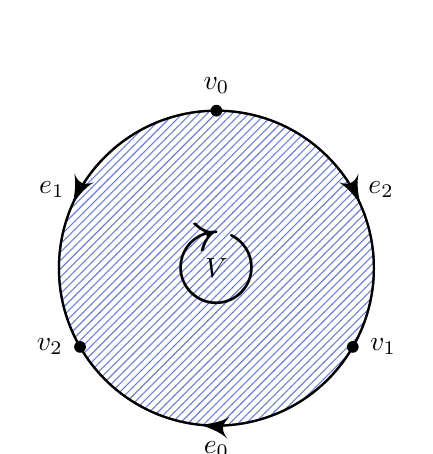
\begin{tikzpicture}[scale=2]
      \draw[pattern=north east lines,opacity=0.7,pattern color=mblue]
        (0,0) circle (1cm) {};
      \draw[->-={2*pi/7}] (90:1) arc[start angle=90, end angle=-30, radius=1];
      \draw[->-={2*pi/7}] (-30:1) arc[start angle=-30, end angle=-150, radius=1];
      \draw[-<-={2*pi/7}] (-150:1) arc[start angle=-150, end angle=-270, radius=1];
      \node[fill, circle, inner sep=1.5pt, label=above:$v_0$] (v0) at (90:1) {};
      \node[fill, circle, inner sep=1.5pt, label=right:$v_1$]
        (v1) at (-30:1) {};
      \node[fill, circle, inner sep=1.5pt, label=left:$v_2$]
        (v2) at (-150:1) {};
      \node[inner sep=1.5pt, label=below:$e_0$] (e0) at (-90:1) {};
      \node[inner sep=1.5pt, label=left:$e_1$] (e1) at (150:1) {};
      \node[inner sep=1.5pt, label=right:$e_2$] (e2) at (30:1) {};
      \node[label=center:$V$] (V) at (0:0) {};
      \node[label=center:{\scalebox{4}{$\circlearrowright$}}]
        (circ) at (0,0) {};
    \end{tikzpicture}
  \end{center}
  We have that
  \begin{align*}
    C_0(\D^2) &= \Z v_0 \oplus \Z v_1 \oplus \Z v_2, \\
    C_1(\D^2) &= \Z e_0 \oplus \Z e_1 \oplus \Z e_2, \\
    C_2(\D^2) &= \Z V.
  \end{align*}
  Therefore we need to compute the homology of a chain complex of the form:
  \[\begin{tikzcd}[ampersand replacement=\&,cramped]
    0 \& \Z \& {\Z^3} \& {\Z^3} \& 0
    \arrow[from=1-1, to=1-2]
    \arrow["{\partial_2}", from=1-2, to=1-3]
    \arrow["{\partial_1}", from=1-3, to=1-4]
    \arrow[from=1-4, to=1-5]
  \end{tikzcd}\]
  We notice that $\ker \partial_0 \cong \Z^3$ and
  \begin{align*}
    \partial_1(e_0) &= v_2 - v_1 \\
    \partial_1(e_1) &= v_2 - v_0 \\
    \partial_1(e_2) &= v_1 - v_0
  \end{align*}
  so $\im \partial_1 \cong \Z^2$.
  This implies that
  \[
    H_0^{\Delta}(\D^2) =
    \frac{\ker \partial_0}{\im \partial_1} \cong
    \Z.
  \]
  We can also notice that $\ker \partial_1 = \Z\set{e_0 - e_1 + e_2} \cong \Z$.
  Since
  \[
    \partial_2(V) = e_2 + e_0 - e_1,
  \]
  we get that $\im \partial_2 = \Z\set{e_2 + e_0 - e_1} \cong \Z$ so
  \[
    H_1^{\Delta}(\D^2) =
    \frac{\ker \partial_1}{\im \partial_2}
    \cong \set{0}.
  \]
  Since for $n \geq 2$ we get that $\ker \partial_n = \set{0}$ it follows
  that $H_n^{\Delta}(\D^2) = \set{0}$ and so finally:
  \[
    H^{\Delta}_n(\D^2) =
    \begin{cases}
      \Z &n = 0, \\
      \set{0} &n > 0.
    \end{cases}
  \]
\end{solution}

\begin{exercise}
  \label{ex:one-two}
  Let $X$ be the (unique) space with a $2$-dimensional $\Delta$-complex
  with one simplex in each dimension $0$, $1$, $2$.
  Compute its simplicial homologies $H_n^{\Delta}(X)$.
\end{exercise}
\begin{solution}
  The space $X$ is the quotient space $T/\sim$ where $T$
  is simply a triangle and the glueing is as follows
  \begin{center}
    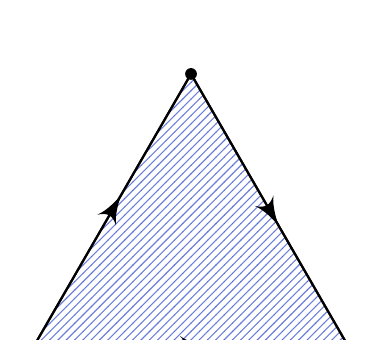
\begin{tikzpicture}[scale=2]
      \draw[pattern=north east lines,opacity=0.7,pattern color=mblue]
        (-1,0) -- (1,0) -- (0,{sqrt(3)}) -- cycle {};
      \draw[-<-={4}] (1,0) -- (-1,0);
      \draw[->-={4}] (-1,0) -- (0,{sqrt(3)});
      \draw[->-={4}] (0,{sqrt(3)}) -- (1,0);
      \node[fill, circle, inner sep=1.5pt]
        (v0) at (0,{sqrt(3)}) {};
      \node[fill, circle, inner sep=1.5pt]
        (v1) at (1,0) {};
      \node[fill, circle, inner sep=1.5pt]
        (v2) at (-1,0) {};
    \end{tikzpicture}
  \end{center}
  and the $\Delta$-complex we construct for it is
  \begin{center}
    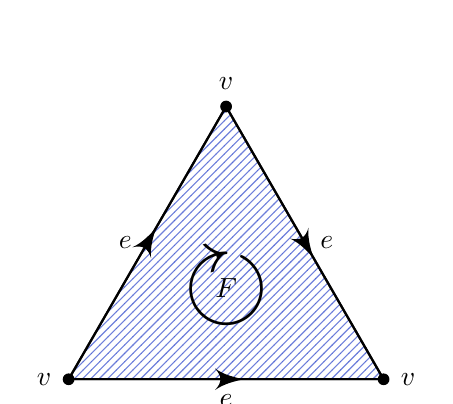
\begin{tikzpicture}[scale=2]
      \draw[pattern=north east lines,opacity=0.7,pattern color=mblue]
        (-1,0) -- (1,0) -- (0,{sqrt(3)}) -- cycle {};
      \draw[-<-={4}] (1,0) -- (-1,0);
      \draw[->-={4}] (-1,0) -- (0,{sqrt(3)});
      \draw[->-={4}] (0,{sqrt(3)}) -- (1,0);
      \node[fill, circle, inner sep=1.5pt, label=above:$v$]
        (v0) at (0,{sqrt(3)}) {};
      \node[fill, circle, inner sep=1.5pt, label=right:$v$]
        (v1) at (1,0) {};
      \node[fill, circle, inner sep=1.5pt, label=left:$v$]
        (v2) at (-1,0) {};
      \node[inner sep=1.5pt, label=left:$e$] (e0) at (-0.5,{sqrt(3)/2}) {};
      \node[inner sep=1.5pt, label=right:$e$] (e1) at (0.5,{sqrt(3)/2}) {};
      \node[inner sep=1.5pt, label=below:$e$] (e2) at (0,0) {};
      \node[label=center:$F$] (F) at (0,{sqrt(1/3)}) {};
      \node[label=center:{\scalebox{4}{$\circlearrowright$}}]
        (circ) at (0,{sqrt(1/3)}) {};
    \end{tikzpicture}
  \end{center}
  and we have that
  \begin{align*}
    C_0(X) &= \Z v, \\
    C_1(X) &= \Z e, \\
    C_2(X) &= \Z F.
  \end{align*}
  Therefore we need to compute the homology of a chain complex of the form:
  \[\begin{tikzcd}[ampersand replacement=\&,cramped]
    0 \& \Z \& {\Z} \& {\Z} \& 0
    \arrow[from=1-1, to=1-2]
    \arrow["{\partial_2}", from=1-2, to=1-3]
    \arrow["{\partial_1}", from=1-3, to=1-4]
    \arrow[from=1-4, to=1-5]
  \end{tikzcd}\]
  We notice that $\ker \partial_0 = \Z v \cong \Z$
  and $\im \partial_1 = \set{0}$.
  Therefore
  \[
    H_0^{\Delta}(X) =
    \frac{\ker \partial_0}{\im \partial_1} =
    \frac{\Z v}{\set{0}} \cong \Z.
  \]
  We also have that $\ker \partial_1 = \Z e \cong \Z$
  and $\im \partial_2 = \Z e \cong \Z$ therefore
  \[
    H_1^{\Delta}(X) =
    \frac{\ker \partial_1}{\im \partial_2} =
    \frac{\Z e}{\Z e} \cong \set{0}.
  \]
  Since for $n \geq 2$ we get that $\ker \partial_n = \set{0}$ it follows
  that $H_n^{\Delta}(X) = \set{0}$ and so finally:
  \[
    H^{\Delta}_n(X) =
    \begin{cases}
      \Z &n = 0, \\
      \set{0} &n > 0.
    \end{cases}
  \]
\end{solution}

\begin{exercise}
  Find a $\Delta$-complex structure to the Klein bottle $K$
  and compute its simplicial homology groups $H_n^{\Delta}(K)$.
\end{exercise}
\begin{solution}
  The $\Delta$-complex we choose is
  \begin{center}
    \begin{tikzpicture}
        \draw[pattern=north west lines,opacity=0.7,pattern color=green] (-2,-2) -- (-2,2) -- (2,2) -- cycle;
        \draw[pattern=dots,opacity=0.7,pattern color=yellow] (-2,-2) -- (2,-2) -- (2,2) -- cycle;
        \draw[->-=4,red] (-2,2) -- (2,2);
        \draw[->-=4,blue] (2,2) -- (2,-2);
        \draw[-<-=4,red] (2,-2) -- (-2,-2);
        \draw[->-=4,blue] (-2,-2) -- (-2,2);
        \draw[->>-={sqrt(32)}] (-2,-2) -- (2,2);
        \node[fill, circle, inner sep=1.5pt, label=left:$v$] (v1) at (-2,-2) {};
        \node[fill, circle, inner sep=1.5pt, label=right:$v$] (v2) at (2,2) {};
        \node[fill, circle, inner sep=1.5pt, label=right:$v$] (v3) at (2,-2) {};
        \node[fill, circle, inner sep=1.5pt, label=left:$v$] (v4) at (-2,2) {};
        \node[label=left:$e$] (e1) at (-2,0) {};
        \node[label=right:$e$] (e2) at (2,0) {};
        \node[label=above:$f$] (f1) at (0,2) {};
        \node[label=below:$f$] (f2) at (0,-2) {};
        \node[label=center:$S$] (S) at (-0.8,0.8) {};
        \node[label=center:$L$] (L) at (0.8,-0.8) {};
        \node[label=below right:$g$] (g) at (-0.2,0.2) {};
        \node[label=center:{\scalebox{4}{$\circlearrowright$}}]
          (circ1) at (0.8,-0.8) {};
        \node[label=center:{\scalebox{4}{$\circlearrowright$}}]
          (circ2) at (-0.8,0.8) {};
    \end{tikzpicture}
  \end{center}
  and we have that
  \begin{align*}
    C_0(K) &= \Z v, \\
    C_1(K) &= \Z e \oplus \Z f \oplus \Z g, \\
    C_2(K) &= \Z S \oplus \Z L.
  \end{align*}
  Therefore we need to compute the homology of a chain complex of the form:
  \[\begin{tikzcd}[ampersand replacement=\&,cramped]
    0 \& \Z^2 \& {\Z^3} \& {\Z} \& 0
    \arrow[from=1-1, to=1-2]
    \arrow["{\partial_2}", from=1-2, to=1-3]
    \arrow["{\partial_1}", from=1-3, to=1-4]
    \arrow[from=1-4, to=1-5]
  \end{tikzcd}\]
  We notice that $\ker \partial_0 = \Z v \cong \Z$
  and $\im \partial_1 = \set{0}$.
  Therefore
  \[
    H_0^{\Delta}(K) =
    \frac{\ker \partial_0}{\im \partial_1} =
    \frac{\Z v}{\set{0}} \cong \Z.
  \]
  We also have that $\ker \partial_1 = \Z e \oplus \Z f \oplus \Z g \cong \Z^3$
  and $\im \partial_2 = \Z \set{e + f - g, g + e - f} \cong \Z^2$ therefore
  \[
    H_1^{\Delta}(K) =
    \frac{\ker \partial_1}{\im \partial_2} =
    \frac{\Z \set{e,f,g}}{\Z \set{e + f - g, g + e - f}}.
  \]
  We see that $\Z \set{e + f - g, g + e - f} = \Z\set{e + f - g, 2f - 2g}$.
  It follows that
  \[
    \frac{\Z \set{e,f,g}}{\Z \set{e + f - g, g + e - f}} =
    \frac{\Z \set{e,f,g}}{\Z \set{e + f - g, 2f - 2g}} =
    \frac{\Z \set{g - f,f,g}}{\Z \set{2f - 2g}} =
    \frac{\Z \set{f,g}}{\Z \set{2f - 2g}}.
  \]
  We now have that
  \[
    H_1^{\Delta}(K) =
    \frac{\Z \set{f,g}}{\Z \set{2f - 2g}} =
    \langle f - g, g \mid 2(f - g) \rangle =
    \langle x, y \mid 2x \rangle \cong \Z \oplus \Z/2\Z.
  \]
  Since for $n \geq 2$ we get that $\ker \partial_n = \set{0}$ it follows
  that $H_n^{\Delta}(K) = \set{0}$ and so finally:
  \[
    H^{\Delta}_n(K) =
    \begin{cases}
      \Z &n = 0, \\
      \Z \oplus \Z/2\Z &n = 1, \\
      \set{0} &n \geq 2.
    \end{cases}
  \]
\end{solution}

\begin{exercise}
  Find a $\Delta$-complex structure for the $n$-sphere $S^n$
  consisting of two $n$-simplices.
  Compute $H_n^{\Delta}(S^n)$ (the homology at dimension $n$).
\end{exercise}
\begin{solution}
  Let $\Delta^n_1$ and $\Delta^n_2$ be two $n$-simplices
  defined by
  \begin{align*}
    \Delta^n_1 &= [v_0,v_1,\dots,v_n] \\
    \Delta^n_2 &= [w_0,w_1,\dots,w_n]
  \end{align*}
  and also glue all their $k$-faces together (this must be done with respect
  to orientation).
  That is, for any subset $\set{i_0,\dots,i_k} \subset \set{0,1,\dots,n}$,
  glue the faces
  $[v_{i_0},v_{i_1},\dots,v_{i_k}]$ and $[w_{i_0},w_{i_1},\dots,w_{i_k}]$.
  Since we know that $\partial \Delta^n \simeq S^{n-1}$,
  and that $\Delta^n \simeq \D^n$, we get that this $\Delta$-complex
  describes two $n$-discs glued at their boundary, which is just $S^n$.
  In order to compute the homology of dimension $n$ we need to find
  \[
    H^{\Delta}_n(S^n) = \frac{\ker \partial_n}{\im \partial_{n+1}},
  \]
  but there are no $\Delta^{n+1}$-simplicies in this $\Delta$-complex,
  so $C_{n+1}(S^n) = \set{0}$ and thus $\im \partial_{n+1} = \set{0}$.
  Let $\sigma_1 \colon \Delta^n_1 \to S^n$
  and $\sigma_2 \colon \Delta^n_2 \to S^n$ be the embeddings of the
  two $n$-simplices in $\R^{n+1}$.
  Since the boundary of $\sigma_1$ and $\sigma_2$ is the same,
  we get that their boundary is equal and then
  $\partial_n(\sigma_1 - \sigma_2) =
    \partial_n(\sigma_1) - \partial_n(\sigma_2) = 0$
  which implies that $\ker \partial_n = \Z\set{\sigma_1 - \sigma_2} \cong \Z$.
  Finally, we get that
  \[
    H^{\Delta}_n(S^n) =
    \frac{\ker \partial_n}{\im \partial_{n+1}} =
    \ker \partial_n \cong \Z.
  \]
\end{solution}

\begin{exercise}
  Find a $\Delta$-complex structure for the space
  $X = \D^2 / e^{it} \sim e^{i(t+2\pi/3)} \forall t\in\R$
  where $\D^2$ is the $2$-disc embedded in $\C$,
  and compute its simplicial homology groups $H_n^{\Delta}(X)$.
\end{exercise}
\begin{solution}
  The space $X$ looks like
  \[
    \tikz[eqpic,scale=2,rotate=-90]{
      \draw[pattern=north east lines,opacity=0.7,pattern color=mblue]
        (0,0) circle (1cm) {};
      \draw[-<-={2*pi/8}] (90:1) arc[start angle=90, end angle=-30, radius=1];
      \draw[-<-={2*pi/7}] (-30:1) arc[start angle=-30, end angle=-150, radius=1];
      \draw[-<-={2*pi/8}] (-150:1) arc[start angle=-150, end angle=-270, radius=1];
      \node[fill, circle, inner sep=1.5pt] (v0) at (90:1) {};
      \node[fill, circle, inner sep=1.5pt]
        (v1) at (-150:1) {};
      \node[fill, circle, inner sep=1.5pt]
        (v2) at (-30:1) {};
      \node[inner sep=1.5pt] (e0 at (-90:1) {};
      \node[inner sep=1.5pt] (e1) at (30:1) {};
      \node[inner sep=1.5pt] (e2) at (150:1) {};
    } \qquad \simeq \quad
    \tikz[eqpic,scale=2]{
      \draw[pattern=north east lines,opacity=0.7,pattern color=mblue]
        (-1,0) -- (1,0) -- (0,{sqrt(3)}) -- cycle {};
      \draw[-<-={4}] (1,0) -- (-1,0);
      \draw[-<-={4}] (-1,0) -- (0,{sqrt(3)});
      \draw[-<-={4}] (0,{sqrt(3)}) -- (1,0);
      \node[fill, circle, inner sep=1.5pt] (v0) at (0,{sqrt(3)}) {};
      \node[fill, circle, inner sep=1.5pt] (v1) at (1,0) {};
      \node[fill, circle, inner sep=1.5pt] (v2) at (-1,0) {};
    }
  \]
  The $\Delta$-complex for $X$ looks like
  \begin{center}
    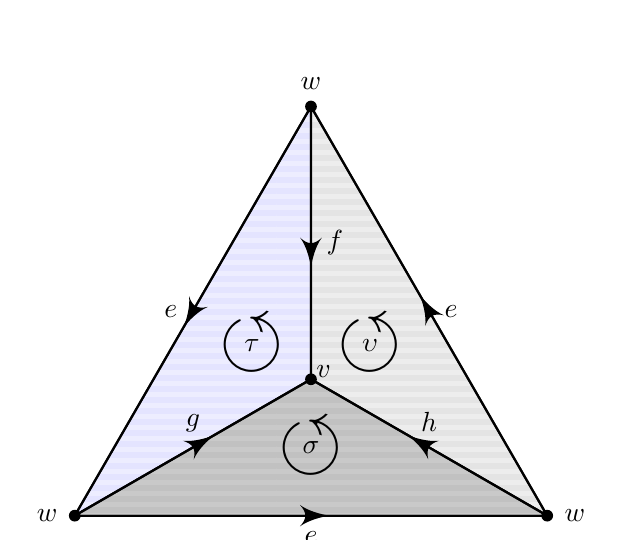
\begin{tikzpicture}[scale=3]
      \draw[pattern=horizontal lines light blue,opacity=0.7,pattern color=mblue]
        (-1,0) -- (0,{sqrt(1/3)}) -- (0,{sqrt(3)}) -- cycle {};
      \draw[pattern=horizontal lines light gray,opacity=0.7,pattern color=mblue]
        (1,0) -- (0,{sqrt(1/3)}) -- (0,{sqrt(3)}) -- cycle {};
      \draw[pattern=horizontal lines gray,opacity=0.7,pattern color=mblue]
        (-1,0) -- (0,{sqrt(1/3)}) -- (1,0) -- cycle {};
      \draw[-<-={6}] (1,0) -- (-1,0);
      \draw[-<-={6}] (-1,0) -- (0,{sqrt(3)});
      \draw[-<-={6}] (0,{sqrt(3)}) -- (1,0);
      \draw[->-={3*sqrt(1+1/3)}] (0,{sqrt(3)}) -- (0,{sqrt(1/3)});
      \draw[->-={3*sqrt(1+1/3)}] (-1,0) -- (0,{sqrt(1/3)});
      \draw[->-={3*sqrt(1+1/3)}] (1,0) -- (0,{sqrt(1/3)});
      \node[fill, circle, inner sep=1.5pt, label=above:$w$]
        (v0) at (0,{sqrt(3)}) {};
      \node[fill, circle, inner sep=1.5pt, label=right:$w$]
        (v1) at (1,0) {};
      \node[fill, circle, inner sep=1.5pt, label=left:$w$]
        (v2) at (-1,0) {};
      \node[inner sep=1.5pt, label=left:$e$] (e0) at (-0.5,{sqrt(3)/2}) {};
      \node[inner sep=1.5pt, label=right:$e$] (e1) at (0.5,{sqrt(3)/2}) {};
      \node[inner sep=1.5pt, label=below:$e$] (e2) at (0,0) {};
      \node[inner sep=1.5pt, label=center:$\sigma$] (sigma)
        at (0,{sqrt(1/3)/2}) {};
      \node[inner sep=1.5pt, label=center:$\tau$] (tau)
        at (-{(sqrt(3)/2)*sqrt(1/3)}/2,{sqrt(1/3)+sqrt(1/3)/4}) {};
      \node[inner sep=1.5pt, label=center:$\upsilon$] (upsilon)
        at ({(sqrt(3)/2)*sqrt(1/3)/2},{sqrt(1/3)+sqrt(1/3)/4}) {};
      \node[label=center:{\scalebox{3}{$\circlearrowleft$}}]
        (circ1) at (0,{sqrt(1/3)/2}) {};
      \node[label=center:{\scalebox{3}{$\circlearrowleft$}}]
        (circ2) at (-{(sqrt(3)/2)*sqrt(1/3)}/2,{sqrt(1/3)+sqrt(1/3)/4}) {};
      \node[label=center:{\scalebox{3}{$\circlearrowleft$}}]
        (circ2) at ({(sqrt(3)/2)*sqrt(1/3)/2},{sqrt(1/3)+sqrt(1/3)/4}) {};
      \node[fill, circle, inner sep=1.5pt, label={[xshift=-1.5mm,yshift=1mm]right:$v$}]
        (v2) at (0,{sqrt(1/3)}) {};
      \node[inner sep=1.5pt, label=right:$f$] (f) at (0,{sqrt(3)-sqrt(1+1/3)/2}) {};
      \node[inner sep=1.5pt, label=above:$g$] (g) at (-0.5,{sqrt(1/3)/2}) {};
      \node[inner sep=1.5pt, label=above:$h$] (h) at (0.5,{sqrt(1/3)/2}) {};
    \end{tikzpicture}
  \end{center}
  We have that
  \begin{align*}
    C_0(X) &= \Z w \oplus \Z v, \\
    C_1(X) &= \Z e \oplus \Z f \oplus \Z g \oplus \Z h, \\
    C_2(X) &= \Z \sigma \oplus \Z \tau \oplus \Z \upsilon.
  \end{align*}
  Therefore we need to compute the homology of a chain complex of the form:
  \[\begin{tikzcd}[ampersand replacement=\&,cramped]
    0 \& \Z^3 \& {\Z^4} \& {\Z^2} \& 0
    \arrow[from=1-1, to=1-2]
    \arrow["{\partial_2}", from=1-2, to=1-3]
    \arrow["{\partial_1}", from=1-3, to=1-4]
    \arrow[from=1-4, to=1-5]
  \end{tikzcd}\]
  We notice that $\ker \partial_0 = \Z v \oplus \Z w \cong \Z^2$
  and $\im \partial_1 = \Z\set{v - w} \cong \Z$.
  Therefore
  \[
    H_0^{\Delta}(X) =
    \frac{\ker \partial_0}{\im \partial_1} =
    \frac{\Z\set{v,w}}{\Z\set{v - w}} =
    \frac{\Z\set{v,v - w}}{\Z\set{v - w}}
  \]
  We also have that $\ker \partial_1 = \Z\set{e,f - g,g - h} \cong \Z^3$
  and after direct calculations of $\partial_2(\sigma)$, $\partial_2(\tau)$
  and $\partial_2(\upsilon)$ we get
  $\im \partial_2 = \Z\set{e + f - h, e + g - f, e + h - g} \cong \Z^3$
  therefore
  \[
    H_1^{\Delta}(X) =
    \frac{\ker \partial_1}{\im \partial_2} =
    \frac{\Z\set{e,f - g,g - h}}{\Z\set{e + f - h, e + g - f, e + h - g}}.
  \]
  We now rewrite the relations using the substitutions
  \[
    \begin{cases}
      x = e, \\
      y = f - g, \\
      x = g - h.
    \end{cases}
  \]
  We get that
  \[
    \frac{\Z\set{e,f - g,g - h}}{\Z\set{e + f - h, e + g - f, e + h - g}} =
    \frac{\Z\set{x,y,z}}{\Z\set{x + y + z, x - y, x - z}}.
  \]
  We have the relations $x = y$ and $x = z$ so this means that the last
  relation is $3x = 0$ so
  \[
    H_1^{\Delta}(X) =
    \frac{\Z\set{x,y,z}}{\Z\set{x + y + z, x - y, x - z}} =
    \frac{\Z\set{x}}{\Z\set{3x}} = \Z/3\Z.
  \]
  Since for $n \geq 2$ we get that $\ker \partial_n = \set{0}$ it follows
  that $H_n^{\Delta}(X) = \set{0}$ and so finally:
  \[
    H^{\Delta}_n(X) =
    \begin{cases}
      \Z &n = 0, \\
      \Z/3\Z &n = 1, \\
      \set{0} &n \geq 2.
    \end{cases}
  \]
\end{solution}

\begin{exercise}
  Find a way to identify pairs of faces of the standard $3$-simplex $\Delta^3$
  to produce a $\Delta$-complex structure for $S^3$.
  Compute its simplicial homology groups $H_n^{\Delta}(S^3)$.
\end{exercise}
\begin{solution}
  In order to visualize $\Delta^3$ we can denote its vertices
  $[v_0,v_1,v_2,v_3]$ and consider the following diagram
  \begin{center}
    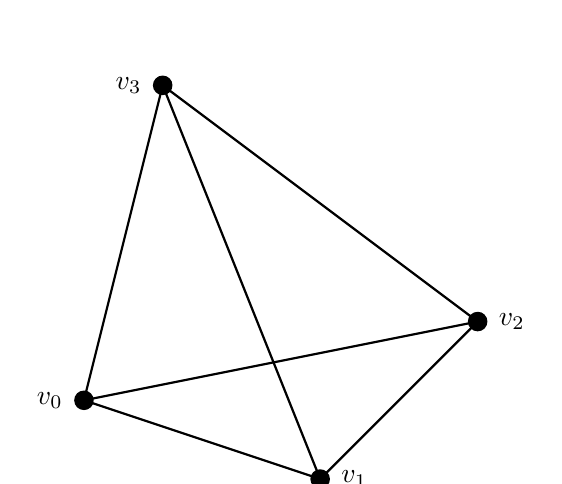
\begin{tikzpicture}
      \node[circle, fill, inner sep=2.5pt, label=left:$v_0$] (v0) at (0,0) {};
      \node[circle, fill, inner sep=2.5pt, label=right:$v_1$] (v1) at (3,-1) {};
      \node[circle, fill, inner sep=2.5pt, label=right:$v_2$] (v2) at (5,1) {};
      \node[circle, fill, inner sep=2.5pt, label=left:$v_3$] (v3) at (1,4) {};
      \draw (0,0) -- (3,-1);
      \draw (0,0) -- (5,1);
      \draw (0,0) -- (1,4);
      \draw (3,-1) -- (5,1);
      \draw (3,-1) -- (1,4);
      \draw (5,1) -- (1,4);
    \end{tikzpicture}
  \end{center}
  As a note, all identification in this question respect the orientation
  (as they must).
  First, we will identify faces $[v_0,v_1,v_3]$ and $[v_2,v_1,v_3]$.
  We shall call this class $\sigma$.
  It induces the identification $[v_0,v_3] \sim [v_2,v_3]$ (which we shall
  call $e_1$), and $[v_0,v_1] \sim [v_2,v_1]$ (which we shall call $e_2$)
  and it identifies $[v_0] \sim [v_2]$ which we shall call $x$.
  This identification of faces gives us a double cone shape with $[v_1]$
  and $[v_3]$ as its antipodal points.
  The double cone shape is homeomorphic to $\D^3$.
  We proceed to identify $[v_0,v_2,v_1]$ and $[v_0,v_2,v_3]$.
  We shall call this class $\tau$.
  This induces the identifications $[v_2,v_1] \sim [v_2,v_3]$ and
  $[v_0,v_1] \sim [v_0,v_3]$
  (so all edges in $e_1$ and $e_2$ are now identified, call this new class
  with $4$ edges $a$).
  This second face identification also induces $[v_1] \sim [v_3]$
  (call this class $y$).
  We now have $2$ unique vertices, $3$ unique edges (denote the edges not
  in class $a$ as $b$ and $c$), two unique faces, and one unique $3$-simplex.
  Finally, we are left with
  \begin{align*}
    &\text{Vertices:} && x = \set{[v_0],[v_2]}, y = \set{[v_1],[v_3]} \\
    &\text{Edges:} && a = \set{[v_0,v_1],[v_0,v_3],[v_2,v_1],[v_2,v_3]},
      b = \set{[v_0,v_2]}, c = \set{[v_1,v_3]} \\
    &\text{Faces:} && \sigma = \set{[v_0,v_1,v_3],[v_2,v_1,v_3]},
      \tau = \set{[v_0,v_2,v_1],[v_0,v_2,v_3]}
  \end{align*}
  Although this is not a very formal justification,
  we can see after identifying the second pair of faces we get $S^3$,
  since they represent the upper and lower hemisphere of $\D^3$
  (which is homeomorphic to the double cone we obtained after the first
  identification), and in any dimension when identifying the lower and upper
  hemispheres of $\D^n$ we get $S^n$.

  In order to compute the homology of this complex we may first
  describe the complex:
  \begin{align*}
    \Delta_0 &= \set{x,y}, \\
    \Delta_1 &= \set{a,b,c}, \\
    \Delta_2 &= \set{\sigma,\tau}, \\
    \Delta_3 &= \set{S}.
  \end{align*}
  For $\partial_1$, we have $\ker \partial_0 = \Z\set{x,y} \cong \Z^2$.
  We also have that
  \begin{align*}
    &\partial_1(a) = \partial_1([v_0,v_1]) = [v_1] - [v_0] = (y) - (x) = y-x \\
    &\partial_1(b) = \partial_1([v_0,v_2]) = [v_2] - [v_0] = (x) - (x) = 0 \\
    &\partial_1(c) = \partial_1([v_1,v_3]) = [v_3] - [v_1] = (y) - (y) = 0
  \end{align*}
  hence $\im \partial_1 = \Z\set{y - x}$ and $\ker \partial_1 = \Z\set{b,c}$
  so in particular
  \[
    H^{\Delta}_0(S^3) =
    \frac{\ker \partial_0}{\im \partial_1} =
    \frac{\Z\set{x,y}}{\Z\set{y - x}} =
    \frac{\Z\set{x,y - x}}{\Z\set{y - x}} \cong \Z.
  \]
  We already found $\ker \partial_1$ so we notice that
  \begin{align*}
    &\partial_2(R) = \partial_2([v_0,v_1,v_3]) =
                  [v_1,v_3] - [v_0,v_3] + [v_0,v_1] = (c) - (a) + (a) = c \\
    &\partial_2(S) = \partial_2([v_0,v_2,v_1]) =
                  [v_2,v_1] - [v_0,v_1] + [v_0,v_2] = (a) - (a) + (b) = b
  \end{align*}
  hence $\im \partial_2 = \Z\set{b,c}$ and $\ker \partial_2 = \set{0}$
  and in particular
  \[
    H^{\Delta}_1(S^3) =
    \frac{\ker \partial_1}{\im \partial_2} =
    \frac{\Z\set{b,c}}{\Z\set{b,c}} \cong \set{0}.
  \]
  We already found $\ker \partial_2$ so we notice that
  \begin{multline*}
    \partial_3(S) = \partial_3([v_0,v_1,v_2,v_3])
      = [v_1,v_2,v_3] - [v_0,v_2,v_3] + [v_0,v_1,v_3] - [v_0,v_1,v_2] \\ =
      (-\sigma) - (\tau) + (\sigma) - (-\tau) = 0,
  \end{multline*}
  hence $\ker \partial_3 = \Z\set{S}$ and $\im \partial_3 = \set{0}$
  and in particular
  \[
    H^{\Delta}_2(S^3) =
    \frac{\ker \partial_2}{\im \partial_3} =
    \frac{\set{0}}{\set{0}} \cong \set{0}.
  \]
  Since there are zero $4$-simplices in the $\Delta$-complex we have
  $\ker \partial_4 = \set{0}$ and thus
  \[
    H^{\Delta}_3(S^3) =
    \frac{\ker \partial_3}{\im \partial_4} =
    \frac{\Z\set{S}}{\set{0}} \cong \Z.
  \]
  For any $n \geq 4$ the map $\partial$ is the zero map and we can
  conclude that
  \[
    H_n^{\Delta}(S^3) =
    \begin{cases}
      \Z &n = 0, \\
      \set{0} &n = 1, \\
      \set{0} &n = 2, \\
      \Z &n = 3, \\
      \set{0} &n \geq 4.
    \end{cases}
  \]
\end{solution}

\begin{exercise}
  Find a simplicial-complex structure for the $2$-torus $T^2$.
  Compute its simplicial homology groups $H_n^{\Delta}(T^2)$.
\end{exercise}
\begin{solution}
  A simplicial structure for $T^2$ is can be described as the following:
  \begin{center}
    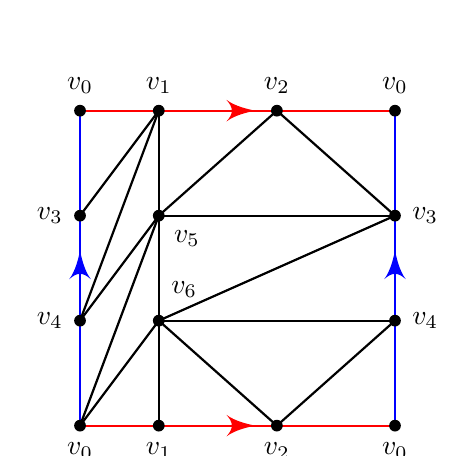
\begin{tikzpicture}[scale=1.0]
        \draw[->-=4,red] (-2,2) -- (2,2);
        \draw[-<-=4,blue] (2,2) -- (2,-2);
        \draw[-<-=4,red] (2,-2) -- (-2,-2);
        \draw[->-=4,blue] (-2,-2) -- (-2,2);
        \node[fill, circle, inner sep=1.5pt, label=below:$v_0$] (v0dl) at (-2,-2) {};
        \node[fill, circle, inner sep=1.5pt, label=below:$v_1$] (v1d) at (-1,-2) {};
        \node[fill, circle, inner sep=1.5pt, label=below:$v_2$] (v2d) at (0.5,-2) {};
        \node[fill, circle, inner sep=1.5pt, label=below:$v_0$] (v0dr) at (2,-2) {};
        \node[fill, circle, inner sep=1.5pt, label=left:$v_4$] (v4l) at (-2,{-2+4/3}) {};
\node[fill, circle, inner sep=1.5pt,
      label={[label distance=2pt]80:$v_6$}] (v6) at (-1,{-2+4/3}) {};
        \node[fill, circle, inner sep=1.5pt, label=right:$v_4$] (v4r) at (2,{-2+4/3}) {};
        \node[fill, circle, inner sep=1.5pt, label=left:$v_3$] (v3l) at (-2,{-2+8/3}) {};
        \node[fill, circle, inner sep=1.5pt, label=below right:$v_5$] (v5) at (-1,{-2+8/3}) {};
        \node[fill, circle, inner sep=1.5pt, label=right:$v_3$] (v3r) at (2,{-2+8/3}) {};
        \node[fill, circle, inner sep=1.5pt, label=above:$v_0$] (v0ul) at (-2,2) {};
        \node[fill, circle, inner sep=1.5pt, label=above:$v_1$] (v1u) at (-1,2) {};
        \node[fill, circle, inner sep=1.5pt, label=above:$v_2$] (v2u) at (0.5,2) {};
        \node[fill, circle, inner sep=1.5pt, label=above:$v_0$] (v0ur) at (2,2) {};
        \draw (v3l.center) -- (v1u.center);
        \draw (v4l.center) -- (v1u.center);
        \draw (v4l.center) -- (v5.center);
        \draw (v0dl.center) -- (v5.center);
        \draw (v0dl.center) -- (v6.center);
        \draw (v1u.center) -- (v5.center);
        \draw (v5.center) -- (v6.center);
        \draw (v6.center) -- (v1d.center);
        \draw (v5.center) -- (v2u.center);
        \draw (v2u.center) -- (v3r.center);
        \draw (v5.center) -- (v3r.center);
        \draw (v6.center) -- (v3r.center);
        \draw (v6.center) -- (v4r.center);
        \draw (v6.center) -- (v2d.center);
        \draw (v2d.center) -- (v4r.center);
    \end{tikzpicture}
  \end{center}
  where the orientation is always by the order of the vertices,
  for example if the face inside the edges $v_5,v_2,v_3$ is mapping
  $[g_1,g_2,g_3]$ to $T^2$, then $g_1 \mapsto v_2$, $g_2 \mapsto v_3$,
  and $g_3 \mapsto v_5$. This is a $\Delta$-complex from pure computation.
  It is a simplicial complex because every edge and every face is determined
  uniquely by its vertices.
  Because I misread the question originally, here is the simplicial homology
  groups for a different non-simplicial $\Delta$-complex.
  A simpler $\Delta$-complex for the $2$-torus (that is not simplicial) is
  \begin{center}
    \begin{tikzpicture}
        \draw[pattern=north west lines,opacity=0.7,pattern color=green] (-2,-2) -- (-2,2) -- (2,2) -- cycle;
        \draw[pattern=dots,opacity=0.7,pattern color=yellow] (-2,-2) -- (2,-2) -- (2,2) -- cycle;
        \draw[->-=4,red] (-2,2) -- (2,2);
        \draw[-<-=4,blue] (2,2) -- (2,-2);
        \draw[-<-=4,red] (2,-2) -- (-2,-2);
        \draw[->-=4,blue] (-2,-2) -- (-2,2);
        \draw[->>-={sqrt(32)}] (-2,-2) -- (2,2);
        \node[fill, circle, inner sep=1.5pt, label=left:$r$] (r1) at (-2,-2) {};
        \node[fill, circle, inner sep=1.5pt, label=right:$r$] (r2) at (2,2) {};
        \node[fill, circle, inner sep=1.5pt, label=right:$r$] (r3) at (2,-2) {};
        \node[fill, circle, inner sep=1.5pt, label=left:$r$] (r4) at (-2,2) {};
        \node[label=left:$e$] (e1) at (-2,0) {};
        \node[label=right:$e$] (e2) at (2,0) {};
        \node[label=above:$f$] (f1) at (0,2) {};
        \node[label=below:$f$] (f2) at (0,-2) {};
        \node[label=center:$V$] (V) at (-0.8,0.8) {};
        \node[label=center:$L$] (L) at (0.8,-0.8) {};
        \node[label=below right:$g$] (g) at (-0.2,0.2) {};
        \node[label=center:{\scalebox{4}{$\circlearrowleft$}}]
          (circ1) at (0.8,-0.8) {};
        \node[label=center:{\scalebox{4}{$\circlearrowright$}}]
          (circ2) at (-0.8,0.8) {};
    \end{tikzpicture}
  \end{center}
  In order to find its simplicial homology groups we first compute the chains:
  \begin{align*}
    C_0(X) &= \Z r, \\
    C_1(X) &= \Z e \oplus \Z f \oplus \Z g, \\
    C_2(X) &= \Z V \oplus \Z L.
  \end{align*}
  Therefore we need to compute the homology of a chain complex of the form:
  \[\begin{tikzcd}[ampersand replacement=\&,cramped]
    0 \& \Z^2 \& {\Z^3} \& {\Z} \& 0
    \arrow[from=1-1, to=1-2]
    \arrow["{\partial_2}", from=1-2, to=1-3]
    \arrow["{\partial_1}", from=1-3, to=1-4]
    \arrow[from=1-4, to=1-5]
  \end{tikzcd}\]
  We notice that $\ker \partial_0 = \Z v \cong \Z$
  and $\im \partial_1 = \set{0}$.
  Therefore
  \[
    H_0^{\Delta}(X) =
    \frac{\ker \partial_0}{\im \partial_1} =
    \frac{\Z v}{\set{0}} \cong \Z.
  \]
  We also have that $\ker \partial_1 = \Z e \oplus \Z f \oplus \Z g \cong \Z^3$
  and $\im \partial_2 = \Z\set{e + f - g} \cong \Z$. Therefore
  \[
    H_1^{\Delta}(X) =
    \frac{\ker \partial_1}{\im \partial_2} =
    \frac{\Z\set{e,f,g}}{\Z\set{e + f - g}} \cong \Z^2.
  \]
  We also have that $\ker \partial_2 = \Z\set{V - L} \cong \Z$ and
  $\im \partial_3 = \set{0}$. Therefore
  \[
    H_2^{\Delta}(X) =
    \frac{\ker \partial_2}{\im \partial_3} =
    \frac{\Z\set{V - L}}{\set{0}} \cong \Z.
  \]
  We see that for $n \geq 3$ we get that $\ker \partial_n = \set{0}$ it follows
  that $H_n^{\Delta}(X) = \set{0}$ and so finally:
  \[
    H^{\Delta}_n(X) =
    \begin{cases}
      \Z &n = 0, \\
      \Z^2 &n = 1, \\
      \Z &n = 2, \\
      \set{0} &n > 2.
    \end{cases}
  \]
\end{solution}


\section{Finitely generated abelian groups}
\begin{exercise}
  Let $f \colon \Z^n \to \Z^m$ be a homomorphism given by
  $f(v) = Av$ where $A$ is an integer matrix.
  Describe an algorithm for computing a (free abelian) basis for $\ker(f)$.
\end{exercise}
\begin{solution}
  We know from the proof of the classification of finitely generated
  abelian groups that $\ker(f) \cong d_1 \Z \oplus \cdots \oplus d_r \Z$
  for some $d_i > 0$ so that $d_i \mid d_{i+1}$ for all $0 < i < r$.
  Our basis is $\set{d_1,d_2,\dots,d_r}$, we just have to find an algorithm
  that finds it.
  Since $\ker(f)$ is a subgroup of $\Z^n$ it is finitely generated.
  Let $k_1,k_2,\dots,k_p$ be generators of $\ker(f)$ and write
  $k_i = (k_{i1},k_{i2},\dots,k_{in})$.
  Set
  \[
    A =
    \begin{pmatrix}
      k_{11} & \cdots & k_{1n} \\
      \vdots & \ddots & \vdots \\
      k_{p1} & \cdots & k_{pn}
    \end{pmatrix}.
  \]
  Notice that when we apply row operations in $\Z$
  (this means we can only multiply rows by $\pm 1$ since these are the only
  invertible elements in $\Z$),
  the rows of the matrix remain a basis for $\ker(f)$,
  and when we apply column operations, the effect is that
  it replaces generators of $\Z^n$ with other generators of $\Z^n$.
  We can see that $\ker(f) = \set{vA \mid v \in \Z^p}$.
  After applying the vector operations (which can be represented
  by multiplying $A$ by some matrix $Q_{n \times n}$ from the left)
  it is clear that $\ker(f) \neq \set{vAQ \mid v \in \Z^p}$,
  however since the column operations are invertible we have a matrix
  $Q^{-1}$ so that $\ker(f) = \set{(vAQ)Q^{-1} \mid v \in \Z^p}$
  which means that the rows of $A$ are still generators of $\ker(f)$
  with respect to other generators of $\Z^n$.
  We want to bring this integer matrix to its Smith normal form:
  \[
    S =
    \begin{pmatrix}
      d_{1} & \cdots & 0 & 0 & \cdots & 0 \\
      \vdots & \ddots & \vdots & \vdots & \ddots & \vdots \\
      0 & \cdots & d_{r} & 0 & \cdots & 0 \\
      0 & \cdots & 0 & 0 & \cdots & 0 \\
      \vdots & \ddots & \vdots & \vdots & \ddots & \vdots \\
      0 & \cdots & 0 & 0 & \cdots & 0
    \end{pmatrix}.
  \]
  It suffices to show that every integer matrix $A$ can be reduced using
  these operations to a matrix of the form
  \[
    \begin{pmatrix}
      d & 0 \\
      0 & B
    \end{pmatrix}
  \]
  where $d$ divides every entery of $B$.
  Call the absolute value of each entry in the matrix its size,
  and call the upper left entry the pivot.
  Now follow the following algorithm:
  \begin{enumerate}
    \item[(step 1)]
      Repeatedly add or subtract the pivot element from other elements
      in the first row and column, until they are of least size.
      The entries now must be either zero,
      or are smaller in size than the pivot.
      In the case there are still nonzero entires,
      change the pivot with the smallest entry, and repeat.
      Since the matrix is finite with integer entries,
      this process must eventually terminate so that all elements in
      the first row and column except the pivot are zero.
    \item[(step 2)]
      If the pivot does not divide every entry of $B$,
      then one of the entries of $B$ has smaller size than the pivot.
      Switch those entries, and repeat step one.
      Otherwise, terminate.
  \end{enumerate}
  This algorithm shows we can being $A$ to its Smith normal form,
  which concludes the proof.
\end{solution}

\begin{exercise} \phantom{}
  \begin{enumerate}
  \item[(1)] Prove that if $A$ is an abelian group such that
    $f \colon A \to \Z^n$  is a surjective homomorphism
    then $A \cong \ker(f) \oplus \Z^n$.
  \item[(2)] Deduce that $H_0(X) \cong \widetilde{H}_0(X) \oplus \Z$.
  \end{enumerate}
\end{exercise}
\begin{solution} \phantom{}
\begin{enumerate}
  \item[(1)]
  This exercise can be solved immediately as a result of the splitting
  lemma, but we have not learned it yet, so we will prove this directly.
  Since $f$ is surjective, there exist $a_1,\dots,a_n \in A$
  so that $f(a_i) = e_i$ for all $i$ where $e_i$ is the $i$th
  element in the standard basis of $\Z^n$.
  We define $g \colon \Z^n \to A$ by $g(e_i) = a_i$ and extend linearly.
  It is clear that $f \circ g = \id$.
  It is clear that the image of $g$ is injective and thus
  $\im(g) \cong \Z^n$.
  It is also clear that $\ker(f) \cap \im(g) = \set{0}$.
  We will show that $A = \ker(f) + \im(g)$.
  For any $a \in A$, denote $b_a := g(f(a)) \in A$.
  We have that $f(a - b_a) = f(a) - f(a) = 0$
  so $a - b_a \in \ker(f)$ and by definition $b_a \in \im(g)$
  so $a = (a - b_a) + b_a$ and $A = \ker(f) + \im(g)$.
  Since $\ker(f) \cap \im(g) = \set{0}$ and $\im(g) \cong \Z^n$
  we get $A \cong \ker(f) \oplus \Z^n$ which completes the first
  part of the exercise.
  \item[(2)]
  Recall that $\widetilde{H}_0(X) = \ker(\epsilon)$
  where $\epsilon \colon C_0(X) \to \Z$ is given by
  $\epsilon(\sum n_i \sigma_i) = \sum n_i$.
  When $X$ is nonempty $\epsilon$ is surjective,
  and then from the result we have
  \[
    C_0(X) \cong \ker(\epsilon) \oplus \Z.
  \]
  We notice that $\im(\partial_1) \subset \ker(\epsilon)$.
  This means that
  \[
    \frac{C_0(X)}{\im(\partial_1)} \cong
    \frac{\ker(\epsilon) \oplus \Z}{\im(\partial_1)} \cong
    \frac{\ker(\epsilon)}{\im(\partial_1)} \oplus \Z,
  \]
  and after recalling the definition of homology and the reduced homology
  we get
  \[
    H_0(X) \cong \widetilde{H}_0(X) \oplus \Z
  \]
  which completes the second part of the proof.
\end{enumerate}
\end{solution}

\begin{exercise}
  Is it true more generally that if $f \colon A \to B$
  is a surjective homomorphism of abelian groups then
  $A \cong \ker(f) \oplus B$?
\end{exercise}
\begin{solution}
  No, the statement is not true in general.
  Consider the function $f \colon \Z \to \Z/2\Z$ given by
  $f(n) = n \pmod{2}$.
  In this case we have that
  \begin{gather*}
    A = \Z \\
    B = \Z/2\Z \\
    \ker(f) = 2\Z
  \end{gather*}
  but $\Z$ is not isomorphic to $2\Z \oplus \Z/2\Z$ since
  $\Z$ is torsion-free and $2\Z \oplus \Z/2\Z$ has torsion.
\end{solution}


\section{Induced maps and homotopy equivalence}

\begin{exercise}
  Prove that $f_{\#} \circ \partial = \partial \circ f_{\#}$.
\end{exercise}
\begin{solution}
  Let $\sigma \in C_n(X)$.
  By the definition of the boundary map we get
  \[
    f_{\#}(\partial \sigma) =
    f_{\#}\del{\sum_{i} (-1)^i \sigma\vert_{[v_0,\dots,\hat v_i,\dots,v_n]}}.
  \]
  Since $f_{\#}$ is defined on basis elements of the chain groups
  and extended linearly we get
  \[
    f_{\#}\del{\sum_{i} (-1)^i \sigma\vert_{[v_0,\dots,\hat v_i,\dots,v_n]}} =
    \sum_{i} (-1)^i f_{\#}\del{\sigma\vert_{[v_0,\dots,\hat v_i,\dots,v_n]}} =
    \sum_{i} (-1)^i f_{\#}(\sigma)\vert_{[v_0,\dots,\hat v_i,\dots,v_n]}.
  \]
  However this is precisely $(\partial \circ f_{\#})(\sigma)$.
  This completes the proof.
\end{solution}

\begin{exercise}
  Prove that the following spaces are homotopy equivalent:
  \begin{enumerate}
    \item[(1)] $\D^n = \set{x \in \R^n \mid \norm{x} \le 1} \simeq
      \R^n \simeq \set{*}$
    \item[(2)] $\D^n \setminus \set{0} \simeq
      \R^n \setminus \set{0} \simeq S^{n-1}$
    \item[(3)] Let $X_{\theta}$ be the space
      \[
        [0,1] \times \set{1,2,3} /
        (0,1) \sim (0,2) \sim (0,3),
        (1,1) \sim (1,2) \sim (1,3)
      \]
      and let $X_8$ be the space
      \[
        [0,1] \times \set{1,2} /
        (0,1) \sim (0,2) \sim (1,1) \sim (1,2)
      \]
      and show that $X_{\theta} \simeq X_8$.
  \end{enumerate}
\end{exercise}
\begin{solution} \phantom{}
  \begin{enumerate}
    \item[(1)] We know that homotopy equivalence is an equivalence relation
      so it suffices to show that $\D^n \simeq \set{*}$ and
      $\R^n \simeq \set{*}$.

      In order to show that $\R^n \simeq \set{*}$ we can choose the maps
      $f \colon \R^n \to \set{*}$ and $g \colon \set{*} \to \R^n$
      as follows
      \begin{align*}
        &f \colon v \mapsto * \\ 
        &g \colon * \mapsto 0 
      \end{align*}
      Since both of these maps are constant they are both continuous.
      We notice that $f \circ g = \id_{\set{*}}$ so in particular
      $f \circ g \simeq \id_{\set{*}}$.
      We have that $g \circ f$ is the zero map.
      We know from topology that $g \circ f$ is homotopic to $\id_{\R^n}$
      by the homotopy $H(x,t) = x \cdot t$.
      This shows that $g \circ f \simeq \id_{\R^n}$ and so
      $f$ is a homotopy equivalence and $\set{*} \simeq \R^n$.

      In order to show that $\D^n \simeq \set{*}$ we can choose the maps
      $f \colon \D^n \to \set{*}$ and $g \colon \set{*} \to \D^n$
      as follows
      \begin{align*}
        &f \colon v \mapsto * \\ 
        &g \colon * \mapsto 0 
      \end{align*}
      Similarly, we get that both of these maps are continuous and
      that $f \circ g \simeq \id_{\set{*}}$.
      We also have that $g \circ f$ is the zero map,
      and the homotopy between $g \circ f$ and $\id_{\D^n}$
      is $H(x,t) = x \cdot t$.
      This shows that $g \circ f \simeq \id_{\R^n}$ and so
      $f$ is a homotopy equivalence and $\set{*} \simeq \R^n$.
    \item[(2)] Since homotopy equivalence is an equivalence relation
      it suffices to show that $\D^n \setminus \set{0} \simeq S^{n-1}$
      and $\R^n \setminus \set{0} \simeq S^{n-1}$.

      In order to show that $\R^n \setminus \set{0} \simeq S^{n-1}$
      we can choose the maps $f \colon \R^n \setminus \set{0} \to S^{n-1}$
      and $g \colon S^{n-1} \to \R^n \setminus \set{0}$ as follows
      \begin{align*}
        &f \colon v \mapsto \frac{v}{\norm{v}} \\ 
        &g \colon e^{it} \mapsto e^{it} 
      \end{align*}
      We notice that $f \circ g = \id_{S^{n-1}}$ and in particular
      we get $f \circ g \simeq \id_{S^{n-1}}$.
      The map $g \circ f$ is simply the map that takes
      $v$ to $\frac{v}{\norm{v}}$.
      The homotopy between $g \circ f$ and $\id_{\R^n \setminus \set{0}}$
      is
      \[
        H(x,t) = \frac{v}{1 + t\del{\norm{v} - 1}}
      \]
      so $g \circ f \simeq \id_{\R^n \setminus \set{0}}$ which implies
      that $\R^n \setminus \set{0} \simeq S^{n-1}$.

      In order to show that $\D^n \setminus \set{0} \simeq S^{n-1}$
      we can use the exact same function and the exact same arguemnts,
      except maybe we also need to show that the homotopy is well defined.
    \item[(3)] First in order to get an intuitive feeling for the spaces
      we draw them.
      We have
      \[
        X_{\theta} =
        \tikz[eqpic,scale=1.5]{
          \draw (0,1) -- (1,1);
          \draw (0,2) -- (1,2);
          \draw (0,3) -- (1,3);
          \node[fill, circle, inner sep=1.5pt, label=above:{$(0,1)$}]
            (a) at (0,1) {};
          \node[fill, circle, inner sep=1.5pt, label=above:{$(0,2)$}]
            (b) at (0,2) {};
          \node[fill, circle, inner sep=1.5pt, label=above:{$(1,1)$}]
            (c) at (1,1) {};
          \node[fill, circle, inner sep=1.5pt, label=above:{$(1,2)$}]
            (d) at (1,2) {};
          \node[fill, circle, inner sep=1.5pt, label=above:{$(0,3)$}]
            (e) at (0,3) {};
          \node[fill, circle, inner sep=1.5pt, label=above:{$(1,3)$}]
            (f) at (1,3) {};
          } \overbrace{\taking{(0,1) \sim (0,2) \sim (0,3)}}^{v}
        \tikz[eqpic,scale=1]{
          \draw (0,0) to[bend left=30] (1,1);
          \draw (0,0) to[bend right=30] (1,-1);
          \draw (0,0) -- (1,0);
          \node[fill, circle, inner sep=1.5, label=left:$v$] (v) at (0,0) {};
          \node[fill, circle, inner sep=1.5pt, label=right:{$(1,3)$}]
            (a) at (1,1) {};
          \node[fill, circle, inner sep=1.5pt, label=right:{$(1,2)$}]
            (b) at (1,0) {};
          \node[fill, circle, inner sep=1.5pt, label=right:{$(1,1)$}]
            (c) at (1,-1) {};
        } \overbrace{\taking{(1,1) \sim (1,2) \sim (1,3)}}^{w}
        \tikz[eqpic,scale=1]{
          \draw (90:1) arc[start angle=90, end angle=-270, radius=1];
          \draw (-1,0) -- (1,0);
          \node[fill, circle, inner sep=1.5, label=left:$v$] (v) at (-1,0) {};
          \node[fill, circle, inner sep=1.5, label=right:$w$] (w) at (1,0) {};
        }
      \]
      and
      \[
        X_{8} =
        \tikz[eqpic,scale=2]{
          \draw (0,1) -- (1,1);
          \draw (0,2) -- (1,2);
          \node[fill, circle, inner sep=1.5pt, label=above:{$(0,1)$}]
            (a) at (0,1) {};
          \node[fill, circle, inner sep=1.5pt, label=above:{$(0,2)$}]
            (b) at (0,2) {};
          \node[fill, circle, inner sep=1.5pt, label=above:{$(1,1)$}]
            (c) at (1,1) {};
          \node[fill, circle, inner sep=1.5pt, label=above:{$(1,2)$}]
            (d) at (1,2) {};
          } \overbrace{\taking{(0,1) \sim (0,2) \sim (1,2) \sim (1,1)}}^{x}
        \tikz[eqpic,scale=1]{
          \draw (90:1) arc[start angle=90, end angle=-270, radius=1];
          \draw (90:-1) arc[start angle=90, end angle=-270, radius=1];
          \node[fill, circle, inner sep=1.5, label=above:$x$] (x) at (0,-1) {} 
        }
      \]
      We won't define the maps rigorously but we can define
      $f \colon X_{\theta} \to X_8$ by mapping the upper semicircle minus
      $v$,$w$ to the upper circle minus $x$,
      the lower semicirlce minus $v$, $w$ to the lower circle 
      minus $x$ and the line segment $[v,w]$ to $x$.
      \[
        \tikz[eqpic,scale=1]{
          \draw[red] (0:1) arc[start angle=0, end angle=180, radius=1];
          \draw[blue] (180:1) arc[start angle=180, end angle=360, radius=1];
          \draw (-1,0) -- (1,0);
          \node[fill, circle, inner sep=1.5, label=left:$v$] (v) at (-1,0) {};
          \node[fill, circle, inner sep=1.5, label=right:$w$] (w) at (1,0) {};
        } \taking{\quad f \quad}
        \tikz[eqpic,scale=1]{
          \draw[red] (90:1) arc[start angle=90, end angle=-270, radius=1];
          \draw[blue] (90:-1) arc[start angle=90, end angle=-270, radius=1];
          \node[fill, circle, inner sep=1.5, label=above:$x$] (x) at (0,-1) {} 
        }
      \]
      We define $g \colon X_8 \to X_{\theta}$ mapping $x$ to the middle
      point on the line segment $[v,w]$ and we map the upper circle minus $v$ to
      the loop based at $x$ going once through the upper semicircle,
      the lower circle minus $v$ to the loop based at $x$ going once
      through the lower semicircle.
      \[
        \tikz[eqpic,scale=1]{
          \draw[red] (90:1) arc[start angle=90, end angle=-270, radius=1];
          \draw[blue] (90:-1) arc[start angle=90, end angle=-270, radius=1];
          \node[fill, circle, inner sep=1.5, label=above:$x$] (x) at (0,-1) {}; 
        } \taking{\quad g \quad}
        \tikz[eqpic,scale=1]{
          \draw[red] (0:1) arc[start angle=0, end angle=180, radius=1];
          \draw[blue] (180:1) arc[start angle=180, end angle=360, radius=1];
          \draw[
        red,
        dash pattern=on 1mm off 1mm,
        postaction={draw, blue, dash phase=1mm, dash pattern=on 1mm off 1mm}
    ] (-1,0) -- (1,0);
          \node[fill, circle, inner sep=1.5, label=above:$x$] (x) at (0,0) {};
        }
      \]
      We have that $f \circ g \simeq \id_{X_8}$
      and $g \circ f \simeq \id_{X_\theta}$ so $f$ is an homotopy equivalence
      between $X_8$ and $X_{\theta}$, which completes the proof.
  \end{enumerate}
    Another way to solve this exercise is by proving that both spaces
    are deformation retracts of a $2$-disc with two holes.
\end{solution}

\begin{exercise}
  Let $A \subseteq X$ be a retract.
  Show that if $X \simeq \set{*}$ then $A \simeq \set{*}$.
\end{exercise}
\begin{solution}
  Since $A$ is a retract there exists a continuous map
  $r \colon X \to A$ so that $r\vert_A = \id_A$.
  Since $X$ is contractible, there exists a homotopy
  $H \colon X \times [0,1] \to X$ so that
  $H(x,0) = x$ is the identity map on $X$
  and $H(x,1) = c$ for some constant $c \in X$.
  In order to show that $A$ is contractible we can define the map
  $H_A \colon A \times [0,1] \to A$ as
  \[
    H_A(a,t) = r(H(a,t)).
  \]
  In this was we have that when $t = 0$
  \[
    H_A(a,0) =
    r(H(a,0)) =
    r(a) = a
  \]
  so $H_A(a,0) = a$ is the identity map on $A$ and when $t = 1$
  we have
  \[
    H_A(a,1) =
    r(H(a,1)) =
    r(c)
  \]
  where $r(c)$ is some constant in $A$.
  Since $H_A$ is a composition of continuous maps, it is continuous,
  and thus it is a homotopy between $A$ and $\set{r(c)}$ so
  $A$ is contractible which completes the proof.
\end{solution}

\begin{exercise}
 Show that if $X \simeq Y$ then $H_n(X) \simeq H_n(Y)$.
\end{exercise}
\begin{solution}
  Since $X$ and $Y$ are homotopy equivalent there exist $f \colon X \to Y$
  and $g \colon Y \to X$ so that $f \circ g \simeq \id_Y$ and
  $g \circ f \simeq \id_X$.
  Consider the induced homomorphisms $f_* \colon H_n(X) \to H_n(Y)$
  and $g_* \colon H_n(Y) \to H_n(X)$.
  From the functoriality of induced maps we get
  \begin{gather*}
    f_* \circ g_* = (f \circ g)_* \\
    g_* \circ f_* = (g \circ f)_*
  \end{gather*}
  and since homotopy equivalent maps induce the same
  homomophism on the homology groups we get
  \begin{gather*}
    f_* \circ g_* = (f \circ g)_* = (\id_Y)_* \\
    g_* \circ f_* = (g \circ f)_* = (\id_X)_*
  \end{gather*}
  which means that the induced maps of the identity maps are simply the identity
  maps of $H_n(X)$ and $H_n(Y)$,hence we have found
  an inverse homomorphism $g_*$ to $f_*$ so $f_*$ must be an isomorphism,
  which means that $H_n(X) \simeq H_n(Y)$ and completes the proof.
\end{solution}

\begin{exercise}
  Let $X$ be the space from \Cref{ex:one-two}.
  Show that $X \simeq \set{*}$.
\end{exercise}
\begin{solution}
  Recall that we are working with the space:
  \[
    \tikz[eqpic,scale=2]{
      \draw[pattern=north east lines,opacity=0.7,pattern color=mblue]
        (-1,0) -- (1,0) -- (0,{sqrt(3)}) -- cycle {};
      \draw[->-={4}] (1,0) -- (-1,0);
      \draw[-<-={4}] (-1,0) -- (0,{sqrt(3)});
      \draw[-<-={4}] (0,{sqrt(3)}) -- (1,0);
      \node[fill, circle, inner sep=1.5pt] (v0) at (0,{sqrt(3)}) {};
      \node[fill, circle, inner sep=1.5pt] (v1) at (1,0) {};
      \node[fill, circle, inner sep=1.5pt] (v2) at (-1,0) {};
    } \quad \simeq \quad
    \tikz[eqpic,scale=2,rotate=-90]{
      \draw[pattern=north east lines,opacity=0.7,pattern color=mblue]
        (0,0) circle (1cm) {};
      \draw[->-={2*pi/8}] (90:1) arc[start angle=90, end angle=-30, radius=1];
      \draw[-<-={2*pi/7}] (-30:1) arc[start angle=-30, end angle=-150, radius=1];
      \draw[-<-={2*pi/8}] (-150:1) arc[start angle=-150, end angle=-270, radius=1];
      \node[fill, circle, inner sep=1.5pt] (v0) at (90:1) {};
      \node[fill, circle, inner sep=1.5pt]
        (v1) at (-150:1) {};
      \node[fill, circle, inner sep=1.5pt]
        (v2) at (-30:1) {};
      \node[inner sep=1.5pt] (e0 at (-90:1) {};
      \node[inner sep=1.5pt] (e1) at (30:1) {};
      \node[inner sep=1.5pt] (e2) at (150:1) {};
    }
  \]
  We notice that this space is simply the space
  \[
    X =
    \D^2 \sqcup_f S^1 := \D^2 \sqcup S^1 / \sim_f
  \]
  where $x \sim_f f(x)$ for $f \colon S^1 \to \D^2$ defined by
  \[
    f\left(e^{2 \pi i t}\right) :=
    \begin{cases}
      e^{2 \pi i (3t)} &t \in [0,1/3], \\
      e^{2 \pi i (3t - 1)} &t \in [1/3,2/3], \\
      e^{-2 \pi i (3t - 2)} &t \in [2/3,1].
    \end{cases}
  \]
  This map wraps a third of the circle over the entire boundary of the disc
  once, then it does the same to the third after it, and finally
  it wraps the last third around the boundary in the opposite direction.
  We will now show
  that $f$ is homotopic to the identity map $i \colon S^1 \to S^1$.
  Define the map
  \[
    \theta(t) :=
    \begin{cases}
      3t &t \in [0,1/3], \\
      3t - 1 &t \in [1/3,2/3], \\
      -(3t - 2) &t \in [2/3,1].
    \end{cases}
  \]
  We can then define the map
  \[
    H(t,s) := e^{2\pi i}\del{(1-s) \theta(t) + s t}.
  \]
  Clearly this is a homotopy between $f$ and the identity of $S^1$
  so we can write $f \simeq \id$.
  We can use this homotopy to construct
  a homotopy equivalence between the spaces
  $\D^2 \sqcup_f S^1$ and $\D^2 \sqcup_{\id} S^1$,
  but it would be more efficient to notice that these are mapping cones,
  and to show that homotopic maps always have homotopy equivalent mapping cones.
  I will add this to the notes.
  Since clearly $\D^2 \sqcup_{\id} S^1$ is simply the disc,
  we get $X \simeq \D^2 \simeq \set{*}$
  and so it is contracible.
\end{solution}


\section{Long exact sequences}

\begin{exercise}
  For $n \geq 1$,
  is the quotient map $q \colon \Delta^n \to \Delta^n / \partial \Delta^n
  \cong S^n$ a generator for $\widetilde H_n(S^n)$?
  Explain how your answer fits with the isomorphism
  $\widetilde H_n(\Delta^n / \partial \Delta^n) \cong
    H_n(\Delta^n,\partial \Delta^n)$.
\end{exercise}
\begin{solution}
  For $n \in 2\N$, denote $\partial_n(\sigma) = \tilde \sigma \in C_{n-1}(X)$.
  We then have that $\tilde \sigma \colon \Delta^{n-1} \to S^n$ is the
  constant map $\tilde \sigma \colon x \mapsto \set{*}$.
  That is because by definition
  \[
    \partial_n(\sigma) :=
    \sum_{i=0}^{n} (-1)^{i} \sigma\vert_{\face{i}} \overset{n\text{ even}}{=}
    \sigma\vert_{[v_0,\dots,v_{n-1}]} := * \neq 0.
  \]
  Therefore $\sigma \notin \ker \partial_n$,
  so $\sigma$ is not even a cycle, so it is definitely not a generator
  for $\widetilde H_n(S^n)$.

  When $n \in 2\N + 1$ then by the same definition for boundary we get
  \[
    \partial_n(\sigma) :=
    \sum_{i=0}^{n} (-1)^{i} \sigma\vert_{\face{i}} \overset{n\text{ odd}}{=}
    0.
  \]
  Therefore $\sigma$ is a cycle and we claim it's a generator.
  We have shown in class that $\id \colon \Delta^n \to \Delta^n$ is a generator
  for $H_n(\Delta^n,\partial \Delta^n)$,
  and since $(\Delta^n,\partial \Delta^n)$ is a good pair,
  the induced map $q_*$ from the quotient map
  $q \colon (\Delta^n,\partial \Delta^n) \to (\Delta^n/\partial \Delta^n,\partial \Delta^n/\partial \Delta^n)$
  is an isomorphism in homology.
  This means that $q_*([\id]) = [q]$
  generates $H_n(\Delta^n/\partial \Delta^n,\partial \Delta^n/\partial \Delta^n)$.

  Next, from the long exact sequence theorem for the good pair
  $(\Delta^n/\partial \Delta^n,\partial \Delta^n/\partial \Delta^n)$,
  we can extract the following short sequence:
  \[\begin{tikzcd}[ampersand replacement=\&,cramped]
    {\widetilde H_n(\partial\Delta^n/\partial\Delta^n)} \& {\widetilde H_n(\Delta^n/\partial\Delta^n)} \& {\widetilde H_n(\Delta^n/\partial\Delta^n,\partial\Delta^n/\partial\Delta^n)} \& {\widetilde H_n(\partial\Delta^n/\partial\Delta^n)}
    \arrow[from=1-1, to=1-2]
    \arrow["{j_*}", from=1-2, to=1-3]
    \arrow[from=1-3, to=1-4]
  \end{tikzcd}\]
  where both ends are trivial, and $j_*$ is induced by the quotient map
  \[\begin{tikzcd}[ampersand replacement=\&,cramped]
    {C_n(\Delta^n/\partial\Delta^n)} \& {C_n(\Delta^n/\partial\Delta^n)/C_n(\partial\Delta^n/\partial\Delta^n)}
    \arrow["j", from=1-1, to=1-2]
  \end{tikzcd}\]
  This means that $j(\sigma) = [q]$, so $j_*(\sigma) = [[q]]$
  which is a generator in homology of the right hand side,
  so $\sigma$ is a generator in homology
  of the left hand side which completes the proof.
\end{solution}

\begin{exercise}
  Give a geometric explanation for the exactness of the long exact sequence
  of the pair $(X,A)$.
\end{exercise}
\begin{solution}
  The long exact sequence of the pair $(X,A)$ is
  \[\begin{tikzcd}[ampersand replacement=\&,cramped]
    \cdots \& {H_n(A)} \& {H_n(X)} \& {H_n(X,A)} \& {H_{n-1}(A)} \& \cdots
    \arrow["\partial", from=1-1, to=1-2]
    \arrow["{i_*}", from=1-2, to=1-3]
    \arrow["{j_*}", from=1-3, to=1-4]
    \arrow["\partial", from=1-4, to=1-5]
    \arrow["{i_*}", from=1-5, to=1-6]
  \end{tikzcd}\]
  and we know what all of these maps are.
  \begin{description}
    \item[($\im i_* = \ker j_*$)]
      The elements of $\im i_*$ are simply cycles in $X$ contained in $A$,
      and the elements in $\ker j_*$ are just cycles in $X$ that are relative
      boundaries in $H_n(X,A)$, but are by definition exactly the same cycles.
      That means that $\im i_* = \ker j_*$.
    \item[($\im j_* \supset \ker \partial$)] Recall that any relative cycle
      in $H_n(X,A)$ can be represented by $\alpha \in C_n(X)$ so that
      $\partial \alpha \in C_{n-1}(A)$.
      Therefore $\ker \partial$ are all the relative cycles so that their
      boundary is also a boundary of an $n$-chain $a \in C_{n-1}(A)$.
      Notice that $\alpha - a \in C_n(X)$,
      and that $j_*([\alpha - a]) = [\alpha]$.
      Therefore $\alpha \in \im j_*$ and thus $\im j_* \supset \ker \partial$.
    \item[($\im j_* \subset \ker \partial$)]
      If $[c] \in H_n(X)$ is a homology class then $j_*([c]) = [c + H_n(A)]$,
      which necessarily includes a chain completely outside $A$,
      therefore $\partial(j_*([c])) = 0$,
      so $\im j_* \subset \ker \partial$.
    \item[($\ker i_* \subset \im \partial$)]
      The elements in $\ker i_*$ are the $(n-1)$-cycles contained in $A$,
      that are the boundaries of some $n$-chain in $X$,
      so therefore $\ker i_* \subset \im \partial$.
    \item[($\ker i_* \supset \im \partial$)]
      Given $\beta \in \im \partial$, then $\beta$ is a boundary in $X$,
      so its homology class in $H_{n-1}(X)$ is zero.
      This means that $i_*(\beta) = 0$ and so $\ker i_* \supset \im \partial$.
  \end{description}
\end{solution}

\begin{exercise}
  The cone $C(X)$ of a topological space $X$ is the space
  $C(X) = X \times [0,1] / X \times \set{1}$.
  Prove that $C(S^1)$ is not homeormophic to $C(S^1 \vee S^1)$.
\end{exercise}
\begin{solution}
  The two spaces we have are
  \[
    C(S^1) =
    \tikz[eqpic,scale=0.5]{
    \draw (-2,0) arc [start angle=180, end angle=360, x radius=2cm, y radius=0.35cm];
    \draw[dashed] (2,0) arc [start angle=0, end angle=180, x radius=2cm, y radius=0.35cm];
    \draw (-2,0) -- (0,4) -- (2,0);
    \node[circle, fill, inner sep=1.5] (a) at (0,4) {};
    } \tand
    C(S^1 \vee S^1) =
    \tikz[eqpic,scale=0.5]{
    \draw (-2,0) arc [start angle=180, end angle=360, x radius=2cm, y radius=0.35cm];
    \draw[dashed] (2,0) arc [start angle=0, end angle=180, x radius=2cm, y radius=0.35cm];
    \draw (-2,0) .. controls (-0.3,2.4) .. (2,4);
    \draw (2,0) .. controls (1,1) and (1,3) .. (2,4);
    \node[circle, fill, inner sep=1.5] (a) at (2,4) {};
    \draw (2,0) arc [start angle=180, end angle=360, x radius=2cm, y radius=0.35cm];
    \draw[dashed] (6,0) arc [start angle=0, end angle=180, x radius=2cm, y radius=0.35cm];
    \draw (2,0) .. controls (3,1) and (3,3) .. (2,4);
    \draw (6,0) .. controls (4.3,2.4) .. (2,4);
    \node[circle, fill, inner sep=1] (b) at (2,0) {};
    }
  \]
  Assume, by way of contradiction, that $f \colon C(S^1 \vee S^1) \to C(S^1)$
  is a homeomorphism.
  Now take out of both spaces the points $(x,1) \in C(S^1 \vee S^1)$
  and $f(x,1) \in C(S^1)$.
  We get something like:
  \[
    C(S^1) =
    \tikz[eqpic,scale=0.5]{
    \draw (-2,0) arc [start angle=180, end angle=360, x radius=2cm, y radius=0.35cm];
    \draw[dashed] (2,0) arc [start angle=0, end angle=180, x radius=2cm, y radius=0.35cm];
    \node (top) at (0,4) {};
    \draw (-2,0) -- (top);
    \draw (top) -- (2,0);
    } \tand
    C(S^1 \vee S^1) =
    \tikz[eqpic,scale=0.5]{
    \draw (-2,0) arc [start angle=180, end angle=360, x radius=2cm, y radius=0.35cm];
    \draw[dashed] (2,0) arc [start angle=0, end angle=180, x radius=2cm, y radius=0.35cm];
    \node (top) at (2,4) {};
    \draw (-2,0) .. controls (-0.3,2.4) .. (top);
    \draw (2,0) .. controls (1,1) and (1,3) .. (top);
    \draw (2,0) arc [start angle=180, end angle=360, x radius=2cm, y radius=0.35cm];
    \draw[dashed] (6,0) arc [start angle=0, end angle=180, x radius=2cm, y radius=0.35cm];
    \draw (2,0) .. controls (3,1) and (3,3) .. (top);
    \draw (6,0) .. controls (4.3,2.4) .. (top);
    \node[circle, fill, inner sep=1] (b) at (2,0) {};
    }
  \]
  but take into account we don't really know which point was $f(x,1)$,
  it could be any point.
  Since the space $C(S^1 \vee S^1) - \set{(x,1)}$ has a deformation retraction
  to $S^1 \vee S^1$ we necessarily get $H_1(C(S^1 \vee S^1) - \set{(x,1)}) = \Z^2$.
  However, we also notice that $C(S^1)$ is simply a $2$-disc
  so $H_1(C(S^1) - \set{f(x,1)})$ is either $\Z$ if $\set{f(x,1)}$ is in the
  interior of the disc and trivial if it is on the boundary of the disc.
  Therefore in any case $H_1(C(S^1) - \set{f(x,1)}) \neq H_1(C(S^1 \vee S^1) - \set{(x,1)})$,
  but since homology is invariant under homeomorphisms, this is a contradiction.
  This contradiction completes the proof.
\end{solution}

\begin{exercise}
  \label{ex:two-four}
  The suspension $S(X)$ of a topological space $X$ is the space
  $S(X) = C(X) / X \times \set{0}$.
  Compute the homologies $\widetilde H_n(S(X))$
  in terms of $\widetilde H_n(X)$.
\end{exercise}
\begin{solution}
  Since the pair $\del{C(x),X \times \set{0}}$ is a good pair,
  we have from the long exact sequence of pairs that:
  \[\begin{tikzcd}[ampersand replacement=\&,cramped]
    {\widetilde H_n(C(X))} \& {\widetilde H_n\left(C(X)/X \times \set{0}\right)} \& {\widetilde H_{n-1}\left(X \times \set{0}\right)} \& {\widetilde H_{n-1}(C(X))}
    \arrow[from=1-1, to=1-2]
    \arrow[from=1-2, to=1-3]
    \arrow[from=1-3, to=1-4]
  \end{tikzcd}\]
  where both ends of the sequence are trivial since $C(X)$ has
  a deformation retraction to a point.
  Therefore $\widetilde H_n\left(C(X)/X \times \set{0}\right) \cong
  \widetilde H_{n-1}\left(X \times \set{0}\right)$,
  and if we recall the definition of a suspension again,
  this is exactly like saying
  $\widetilde H_n(S(X)) \cong \widetilde H_{n-1}(X)$.
\end{solution}

\begin{exercise}
  Use \Cref{ex:two-four} to compute the homologies of $S^n$
  (Hint: what is $S(S^n)$?)
\end{exercise}
\begin{solution}
  Recall that
  \[
    S(S^1) =
    \tikz[eqpic,scale=0.3]{
    \draw (-2,0) arc [start angle=180, end angle=360, x radius=2cm, y radius=0.35cm];
    \draw[dashed] (2,0) arc [start angle=0, end angle=180, x radius=2cm, y radius=0.35cm];
    \draw (-2,0) -- (0,4) -- (2,0);
    \draw (-2,0) -- (0,-4) -- (2,0);
    \node[circle, fill, inner sep=1.5] (a) at (0,4) {};
    \node[circle, fill, inner sep=1.5] (b) at (0,-4) {};
    } \cong S^2
  \]
  and similarly $S(S^n) = S^{n+1}$ for all $n \in \N$.
  Thus, by \Cref{ex:two-four} we get that
  \[
    \widetilde H_n(S^n) =
    \widetilde H_{n-1}(S^{n-1}) = \cdots =
    \widetilde H_0(S^0) = \Z.
  \]
  For $n > m$, we get that
  \[
    \widetilde H_n(S^m) = \cdots =
    \widetilde H_{n - m}(S^0) = 0,
  \]
  and for $n < m$, we similarly get that
  $\widetilde H_n(S^m) = \widetilde H_0(S^{m - n}) = 0$,
  where the last equality stems from the fact $S^{m - n}$ is connected
  for $n < m$.
\end{solution}

\begin{exercise}
  Let $X$ be a topological space
  and let $A \subseteq X$ so that $(A,X)$ is a good pair.
  Consider $Y = X \sqcup C(A) / a \sim (a,0)$ for all $a \in A$.
  Prove that $\widetilde H_n(Y) \cong H_n(X,A)$.
\end{exercise}
\begin{solution}
  Since $C(A)$ is contractible, from the long exact sequecne of
  pairs we get that $\widetilde H_n(Y) \cong H_n(Y,C(A))$.
  By the excision theorem we get that for any $* \in \Int(C(A))$
  the inclusion map $i \colon (X - Z, A - Z) \hookrightarrow (X,A)$ induces
  an isomorphism $H_n(Y,C(A)) \cong H_n(Y - \set{*}, C(A) - \set{*})$
  for all $n \in \N$.
  In particular this is true if $*$ is the apex of the cone $C(A)$.
  Since a cone without its apex has a deformation retraction onto its
  basis, thus there exists a homotopy equivalence of pairs between
  $(Y - \set{*}, C(A) - \set{*})$ and $(X,A)$,
  and thus $H_n(X,A) \cong H_n(Y - \set{*}, C(A) - \set{*})$.
  By composing all of the isomorphisms we have shown so far we can conlude
  that $\widetilde H_n(Y) \cong H_n(X,A)$,
  which completes the proof.
\end{solution}

\begin{exercise}
  \label{ex:two-seven}
  Compute the homologies of the following spaces using the long exact
  sequence of a pair:
  \begin{enumerate}
    \item[(1)] The real projective space $\RP^2$.
    \item[(2)] The two-dimensional torus $T^2 = S^1 \times S^1$.
    \item[(3)] The Klein bottle.
  \end{enumerate}
\end{exercise}
\begin{solution} \phantom{}
  \begin{enumerate}
    \item[(1)] Denote
      \begin{center}
        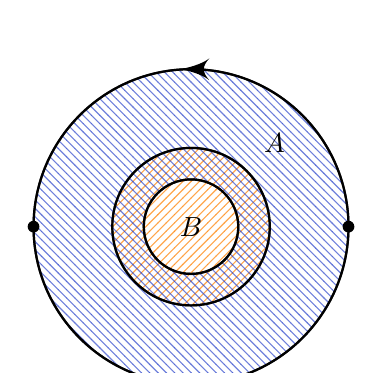
\begin{tikzpicture}[scale=2]
          \draw[pattern=north east lines,opacity=0.7,pattern color=orange]
            (0,0) circle (0.5cm) {};
          \draw[pattern=north west lines, opacity=0.7, pattern color=mblue, even odd rule]
            (0,0) circle (1cm)  % Outer circle
            (0,0) circle (0.3cm);    % Inner circle (subtracted)
          \draw (0:0.5) arc[start angle=0, end angle=360, radius=0.5];
          \draw (0:0.3) arc[start angle=0, end angle=360, radius=0.3];
          \draw[-->]
            (90:1) arc[start angle=90, end angle=270, radius=1];
          \draw[-->]
            (-90:1) arc[start angle=-90, end angle=90, radius=1];
          \node[fill, circle, inner sep=1.5pt] (v0) at (180:1) {};
          \node[fill, circle, inner sep=1.5pt] (v1) at (0:1) {};
          \node[inner sep=1.5pt, label=center:$B$] (B) at (0:0) {};
          \node[inner sep=1.5pt, label=center:$A$] (A) at (45:0.75) {};
        \end{tikzpicture}
      \end{center}
      Note that since the interiors of $A$ and $B$ cover $X := \RP^2$,
      thus by the excision theorem the inclusion map 
      $i \colon (A,A \cap B) \hookrightarrow (X,B)$ induces an isomorphism
      $H_n(A,A \cap B) \cong H_n(A \cup B, B)$.
      Moreover, since $\RP^2 = A \cup B$ and taking the homology of a space
      relative to a point is equivalent to taking the reduced homology of 
      the space we get
      $H_n(A,A \cap B) \cong H_n(A \cup B, B) \cong \widetilde H_n(\RP^2)$.
      Since $(A, A \cap B)$ is a good pair by the long exact sequence
      theorem we have the sequence
    \begin{center}
      \begin{tikzcd}
        \cdots \ar[r] &
        H_2(A,A \cap B) \ar[r] &
        \widetilde H_1(A \cap B) \ar["i_*",r] &
        \widetilde H_1(A) \ar["q_*",out=0, in=180, looseness=2, overlay, lld]\\
        & H_1(A,A \cap B) \ar["\partial_1",r] &
        \widetilde H_0(A) \ar[r] &
        \widetilde H_0(B) \ar [r] & \cdots
      \end{tikzcd}
    \end{center}
    Since $H_2(A,A \cap B) \cong \widetilde H_0(A) \cong \widetilde H_0(B)
    \cong \set{0}$,
    since $H_1(A \cap B) \cong H_1(A) \cong \Z$
    we get an exact sequence of the form
    \begin{center}
      \begin{tikzcd}
        \cdots \ar[r] &
        0 \ar[r] &
        \Z \ar["i_*",r] &
        \Z \ar["q_*",out=0, in=180, looseness=2, overlay, lld]\\
        & H_1(A,A \cap B) \ar["\partial_1",r] &
        0 \ar[r] &
        0 \ar [r] & \cdots
      \end{tikzcd}
    \end{center}
    Since the generator of $\widetilde H_1(A \cap B)$ is two times
    the generator of $\widetilde H_1(A)$ (one lap around $S^1$
    is sent to two laps around $A \cong M$),
    we get $i_*([1]) = [2]$.
    From the exactness of the sequence we get
    $\ker q_* = 2\Z$.
    From exactness again, we get
    \[
      \im q_* = \ker \partial_1 = H_1(A, A \cap B),
    \]
    so $q_*$ is onto, therefore by the first isomorphism theorem for
    groups we have
    \[
      \im q_* =
      \frac{\Z}{\ker q_*} =
      \frac{\Z}{2\Z} =
      H_1(A, A \cap B).
    \]
    Therefore, by all previous calculations we get:
    \[
      \widetilde H_n(\RP^2) =
      \begin{cases}
        \Z/2\Z & n = 1, \\
        0 &\text{otherwise}.
      \end{cases}
    \]
    \item[(2)]
      Denote
      \begin{center}
    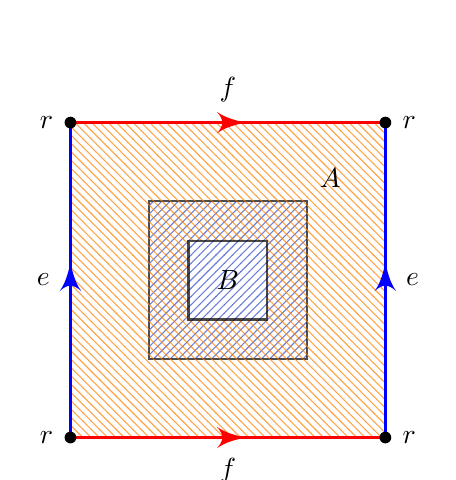
\begin{tikzpicture}
        \draw[pattern=north east lines, opacity=0.7, pattern color=mblue]
          (-1,-1) rectangle (1,1);
        \draw[pattern=north west lines, opacity=0.7, pattern color=orange, even odd rule]
          (-2,-2) rectangle (2,2)        % Outer square
          (-0.5,-0.5) rectangle (0.5,0.5); % Inner square (hole)
        \draw[->-=4,red] (-2,2) -- (2,2);
        \draw[-<-=4,blue] (2,2) -- (2,-2);
        \draw[-<-=4,red] (2,-2) -- (-2,-2);
        \draw[->-=4,blue] (-2,-2) -- (-2,2);
        \node[fill, circle, inner sep=1.5pt, label=left:$r$] (r1) at (-2,-2) {};
        \node[fill, circle, inner sep=1.5pt, label=right:$r$] (r2) at (2,2) {};
        \node[fill, circle, inner sep=1.5pt, label=right:$r$] (r3) at (2,-2) {};
        \node[fill, circle, inner sep=1.5pt, label=left:$r$] (r4) at (-2,2) {};
        \node[label=left:$e$] (e1) at (-2,0) {};
        \node[label=right:$e$] (e2) at (2,0) {};
        \node[label=above:$f$] (f1) at (0,2) {};
        \node[label=below:$f$] (f2) at (0,-2) {};
        \node[label=center:$A$] (A) at (1.3,1.3) {};
        \node[label=center:$B$] (B) at (0,0) {};
    \end{tikzpicture}
  \end{center}
    In this case by the excision theorem we have that
    \[
      \widetilde H_n(T^2) \cong
      H_n(T^2,B) \cong
      H_n(A,A \cap B) \cong
      \widetilde H_n(A,A \cap B).
    \]
    Since the pair $(A \cap B, A)$ is a good pair,
    from the long exact sequence of pairs theorem we get the following
    long exact sequence:
    \begin{center}
      \begin{tikzcd}
        \cdots \ar[r] &
        H_2(A,A \cap B) \ar[r] &
        \widetilde H_1(A \cap B) \ar["i_*",r] &
        \widetilde H_1(A) \ar["q_*",out=0, in=180, looseness=2, overlay, lld]\\
        & H_1(A,A \cap B) \ar["\partial_1",r] &
        \widetilde H_0(A) \ar[r] &
        \widetilde H_0(B) \ar [r] & \cdots
      \end{tikzcd}
    \end{center}
    Since we know that $\widetilde H_1(A \cap B) \cong \Z$
    and since $A$ is homotopy equivalent to the figure
    eight space $S^1 \vee S^1$ as we can see below
    \[
      \tikz[eqpic,scale=0.5]{
        \draw[pattern=north west lines, opacity=0.7, pattern color=orange, even odd rule]
          (-2,-2) rectangle (2,2)        % Outer square
          (-0.5,-0.5) rectangle (0.5,0.5); % Inner square (hole)
        \draw[->-=4,red] (-2,2) -- (2,2);
        \draw[-<-=4,blue] (2,2) -- (2,-2);
        \draw[-<-=4,red] (2,-2) -- (-2,-2);
        \draw[->-=4,blue] (-2,-2) -- (-2,2);
        \node[label=left:$e$] (e1) at (-2,0) {};
        \node[label=right:$e$] (e2) at (2,0) {};
        \node[label=above:$f$] (f1) at (0,2) {};
        \node[label=below:$f$] (f2) at (0,-2) {};
      } \taking{\qquad}
      \tikz[eqpic,scale=0.5]{
        \draw[->-=4,red] (-2,2) -- (2,2);
        \draw[-<-=4,blue] (2,2) -- (2,-2);
        \draw[-<-=4,red] (2,-2) -- (-2,-2);
        \draw[->-=4,blue] (-2,-2) -- (-2,2);
        \node[label=left:$e$] (e1) at (-2,0) {};
        \node[label=right:$e$] (e2) at (2,0) {};
        \node[label=above:$f$] (f1) at (0,2) {};
        \node[label=below:$f$] (f2) at (0,-2) {};
      } \taking{\qquad}
      \tikz[eqpic,scale=1]{
          \draw[red] (90:1) arc[start angle=90, end angle=-270, radius=1];
          \draw[blue] (90:-1) arc[start angle=90, end angle=-270, radius=1];
        \node[label=right:$e$] (e2) at (1,0) {};
        \node[label=right:$f$] (f2) at (1,-2) {};
      }
    \]
    we get that $\widetilde H_1(A) \cong \Z^2$.
    We also know that $\widetilde H_0(A \cap B) \cong \widetilde H_0(A) \cong
    \set{0}$.
    Therefore we have the exact sequence:
    \begin{center}
      \begin{tikzcd}
        \cdots \ar[r] &
        H_2(A,A \cap B) \ar[r] &
        \widetilde \Z \ar["i_*",r] &
        \widetilde \Z^2 \ar["q_*",out=0, in=180, looseness=2, overlay, lld]\\
        & H_1(A,A \cap B) \ar["\partial_1",r] &
        0 \ar[r] &
        0\ar [r] & \cdots
      \end{tikzcd}
    \end{center}
      Recall that $A \cap B$ have a deformation retraction to $S^1$
      and $A$ to $S^1 \vee S^1$ to get
      \[
        \widetilde H_2(T^2) \cong
        H_2(A,A \cap B) \cong
        H_2(S^1 \vee S^1,S^1) = \Z.
      \]
      Notice that $i_*([1]) = [(0,0)]$,
      so $\ker q_* = \im i_* = \set{0}$,
      and also $H_1(A,A \cap B) = \ker \partial_1 = \im q_*$.
      From the first isomorphism theorem for groups,
      we get
      \[
        H_1(A,A \cap B) = \im q_* \cong
        \frac{\Z^2}{\ker q_*} \cong
        \frac{\Z^2}{\set{0}} = \Z^2.
      \]
      Therefore, by all previous calculations we get:
      \[
        \widetilde H_n(T^2) =
        \begin{cases}
          0 & n = 0, \\
          \Z^2 & n = 1, \\
          \Z & n = 2, \\
          0 &\text{otherwise}.
        \end{cases}
      \]
    \item[(3)] Denote
      \begin{center}
      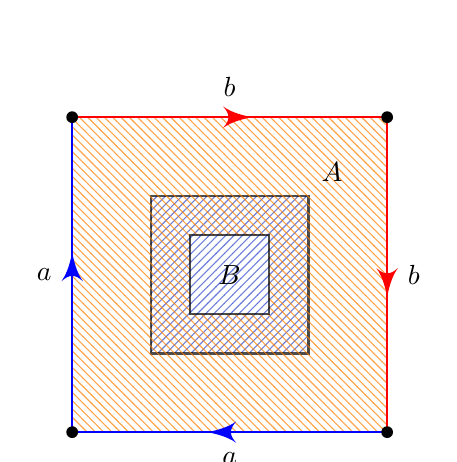
\begin{tikzpicture}
        \draw[pattern=north east lines, opacity=0.7, pattern color=mblue]
          (-1,-1) rectangle (1,1);
        \draw[pattern=north west lines, opacity=0.7, pattern color=orange, even odd rule]
          (-2,-2) rectangle (2,2)        % Outer square
          (-0.5,-0.5) rectangle (0.5,0.5); % Inner square (hole)
        \draw[->-=4/0.8,red] (-2,2) -- (2,2);
        \draw[->-=4/0.8,red] (2,2) -- (2,-2);
        \draw[->-=4/0.8,blue] (2,-2) -- (-2,-2);
        \draw[->-=4/0.8,blue] (-2,-2) -- (-2,2);
        \node[fill, circle, inner sep=1.5pt] (r1) at (-2,-2) {};
        \node[fill, circle, inner sep=1.5pt] (r2) at (2,2) {};
        \node[fill, circle, inner sep=1.5pt] (r3) at (2,-2) {};
        \node[fill, circle, inner sep=1.5pt] (r4) at (-2,2) {};
        \node[label=left:$a$] (a1) at (-2,0) {};
        \node[label=right:$b$] (a2) at (2,0) {};
        \node[label=above:$b$] (b1) at (0,2) {};
        \node[label=below:$a$] (b2) at (0,-2) {};
        \node[label=center:$A$] (A) at (1.3,1.3) {};
        \node[label=center:$B$] (B) at (0,0) {};
      \end{tikzpicture}
      \end{center}
    By the excision theorem we have that
    \[
      H_n(K) \cong
      \widetilde H_n(K,B) \cong
      \widetilde H_n(A,A \cap B) \cong
      H_n(A,A \cap B).
    \]
    We now have a long exact sequence:
    \begin{center}
      \begin{tikzcd}
        \cdots \ar[r] &
        H_2(A,A \cap B) \ar[r] &
        \widetilde H_1(A \cap B) \ar["i_*",r] &
        \widetilde H_1(A) \ar["q_*",out=0, in=180, looseness=2, overlay, lld]\\
        & H_1(A,A \cap B) \ar["\partial_1",r] &
        \widetilde H_0(A) \ar[r] &
        \widetilde H_0(B) \ar [r] & \cdots
      \end{tikzcd}
    \end{center}
    Since $A \cap B \simeq_{\text{dfr}} S^1$
    and $A \simeq_{\text{dfr}} S^1 \vee S^1$,
    and
    $H_2(A,A \cap B) \cong \widetilde H_0(A) \cong \widetilde H_0(A) = \set{0}$
    we get an exact sequence of the form:
    \begin{center}
      \begin{tikzcd}
        \cdots \ar[r] &
        0 \ar[r] &
        \Z \ar["i_*",r] &
        \Z^2 \ar["q_*",out=0, in=180, looseness=2, overlay, lld]\\
        & H_1(A,A \cap B) \ar["\partial_1",r] &
        0 \ar[r] &
        0\ar [r] & \cdots
      \end{tikzcd}
    \end{center}
    We can see that this time $i_*([1]) = ([2,0])$.
    Thus $\ker q_* = \im i_* = 2\Z \times \set{0}$,
    and also $H_1(A,A \cap B) = \ker \partial_1 = \im q_*$.
    From the first isomorphism theorem for groups,
    we get
    \[
      H_1(A,A \cap B) = \im q_* \cong
      \frac{\Z^2}{\ker q_*} \cong
      \frac{\Z^2}{2\Z \times \set{0}} = \Z/2\Z \oplus \Z.
    \]
    Therefore, by all previous calculations we get:
    \[
      \widetilde H_n(K) =
      \begin{cases}
        0 & n = 0, \\
        \Z/2\Z \oplus \Z & n = 1, \\
        0 &\text{otherwise}.
      \end{cases}
    \]
  \end{enumerate}
\end{solution}

\begin{exercise}
  Repeat the previous exercise using Mayer--Vietoris.
\end{exercise}
\begin{solution} \phantom{}
  \begin{enumerate}
    \item[(1)] Consider the space $\RP^2$.
      We can choose $A \cong \D^2$ and $B \cong M$ where $M$ is the M\"obius
      band.
      \begin{center}
        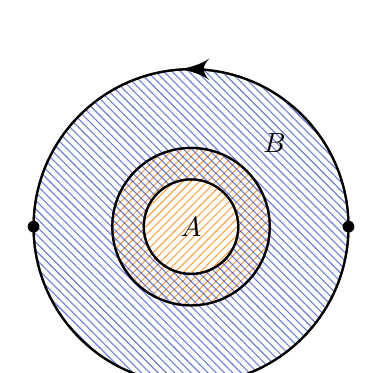
\begin{tikzpicture}[scale=2]
          \draw[pattern=north east lines,opacity=0.7,pattern color=orange]
            (0,0) circle (0.5cm) {};
          \draw[pattern=north west lines, opacity=0.7, pattern color=mblue, even odd rule]
        (0,0) circle (1cm)  % Outer circle
        (0,0) circle (0.3cm);    % Inner circle (subtracted)
          \draw (0:0.5) arc[start angle=0, end angle=360, radius=0.5];
          \draw (0:0.3) arc[start angle=0, end angle=360, radius=0.3];
          \draw[-->]
            (90:1) arc[start angle=90, end angle=270, radius=1];
          \draw[-->]
            (-90:1) arc[start angle=-90, end angle=90, radius=1];
          \node[fill, circle, inner sep=1.5pt] (v0) at (180:1) {};
          \node[fill, circle, inner sep=1.5pt] (v1) at (0:1) {};
          \node[inner sep=1.5pt, label=center:$A$] (A) at (0:0) {};
          \node[inner sep=1.5pt, label=center:$B$] (A) at (45:0.75) {};
        \end{tikzpicture}
      \end{center}
      Then from Mayer--Vietoris we get the following long exact sequence:
      \[
      \begin{tikzcd}
        \cdots \ar[r] & \widetilde H_2(A) \oplus \widetilde H_2(B) \ar[r] & \widetilde H_2(\RP^2) \ar[r] & \widetilde H_1(A \cap B) \ar[out=0, in=180, looseness=2, overlay, lld]\\
        & \widetilde H_1(A) \oplus \widetilde H_1(B) \ar[r] & \widetilde H_1(\RP^2) \ar[r] & \widetilde H_0(A \cap B) \ar [r] & \cdots
      \end{tikzcd}
      \]
      We know that $A$ is contractible
      so $\widetilde H_{1}(A) = \widetilde H_{2}(A) = \set{0}$
      and the M\"obius band has a deformation retraction to $S^1$.
      So does $A \cap B$.
      We now have an exact sequence of the form
      \[\begin{tikzcd}[ampersand replacement=\&,cramped]
        0 \& {\widetilde H_2(\RP^2)} \& \Z \& \Z \& {\widetilde H_1(\RP^2)} \& 0
        \arrow[from=1-1, to=1-2]
        \arrow["\alpha",from=1-2, to=1-3]
        \arrow["\beta",from=1-3, to=1-4]
        \arrow["\gamma",from=1-4, to=1-5]
        \arrow[from=1-5, to=1-6]
      \end{tikzcd}\]
      Since we know what the maps in the Mayer--Vietoris sequence
      are, we can see that $\beta([1]) = [(2,0)]$ (the right $\Z$
      is actuall $\Z \oplus \set{0}$).
      Since $\ker \beta = 0$
      and the sequence is exact we get $\im \alpha = 0$.
      Thus, from the first isomorphism theorem we get
      \[
        0 \cong
        \frac{\widetilde H_2(\RP^2)}{\ker \alpha} \cong
        \frac{\widetilde H_2(\RP^2)}{\im 0} \cong
        \widetilde H_2(\RP^2).
      \]
      Similarly to what we did in \Cref{ex:two-seven} part $(1)$
      we get that $\widetilde H_1(\RP^2) = \Z/2\Z$.
      Therefore, we got the same results
      \[
      \widetilde H_n(\RP^2) =
      \begin{cases}
        \Z/2\Z & n = 1, \\
        0 &\text{otherwise}.
      \end{cases}
      \]
    \item[(2)] Denote
      \begin{center}
    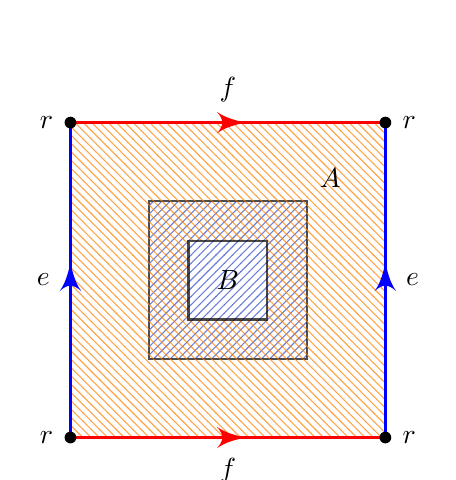
\begin{tikzpicture}
        \draw[pattern=north east lines, opacity=0.7, pattern color=mblue]
          (-1,-1) rectangle (1,1);
        \draw[pattern=north west lines, opacity=0.7, pattern color=orange, even odd rule]
          (-2,-2) rectangle (2,2)        % Outer square
          (-0.5,-0.5) rectangle (0.5,0.5); % Inner square (hole)
        \draw[->-=4,red] (-2,2) -- (2,2);
        \draw[-<-=4,blue] (2,2) -- (2,-2);
        \draw[-<-=4,red] (2,-2) -- (-2,-2);
        \draw[->-=4,blue] (-2,-2) -- (-2,2);
        \node[fill, circle, inner sep=1.5pt, label=left:$r$] (r1) at (-2,-2) {};
        \node[fill, circle, inner sep=1.5pt, label=right:$r$] (r2) at (2,2) {};
        \node[fill, circle, inner sep=1.5pt, label=right:$r$] (r3) at (2,-2) {};
        \node[fill, circle, inner sep=1.5pt, label=left:$r$] (r4) at (-2,2) {};
        \node[label=left:$e$] (e1) at (-2,0) {};
        \node[label=right:$e$] (e2) at (2,0) {};
        \node[label=above:$f$] (f1) at (0,2) {};
        \node[label=below:$f$] (f2) at (0,-2) {};
        \node[label=center:$A$] (A) at (1.3,1.3) {};
        \node[label=center:$B$] (B) at (0,0) {};
    \end{tikzpicture}
    \end{center}
      Then from Mayer--Vietoris we get the following long exact sequence:
      \[
        \begin{tikzcd}
          \cdots \ar[r] &
          \widetilde H_2(T^2) \ar[r] & 
          \widetilde H_1(A \cap B) \ar[r] &
          \widetilde H_1(A) \oplus \widetilde H_1(B)
            \ar[out=0, in=180, looseness=2, overlay, lld]\\
          & \widetilde H_1(T^2) \ar[r]
          & \widetilde H_0(A \cap B) \ar[r]
          & \widetilde H_0(A) \oplus \widetilde H_0(B) \ar [r] & \cdots
        \end{tikzcd}
      \]
      We know that $\widetilde H_0(A) \oplus \widetilde H_0(B)
      \cong \widetilde H_0(A \cap B) \cong \set{0}$.
      We also know that $A \simeq_{\text{dfr}} S^1 \vee S^1$
      so $\widetilde H_1(A) = \Z^2$.
      We also know that $\widetilde H_1(B) = \set{0}$
      and $\widetilde H_1(A \cap B) \cong \Z$.
      Therefore, we can rewrite the diagram as:
      \[
        \begin{tikzcd}[ampersand replacement=\&,cramped]
        \widetilde H_2(T^2) \&
        \Z \& \Z^2 \oplus \set{0} \&
        \widetilde H_1(T^2) \& 0 \& 0
        \arrow["\delta",from=1-1, to=1-2]
        \arrow["\alpha",from=1-2, to=1-3]
        \arrow["\beta",from=1-3, to=1-4]
        \arrow["\gamma",from=1-4, to=1-5]
        \arrow[from=1-5, to=1-6]
        \end{tikzcd}
      \]
      so that $\alpha([1]) = ([(0,0)],0)$.
      From exactness at $\widetilde H_2(T^2)$ we know that
      $\delta$ is injective, and since $\im \delta = \ker \alpha = \Z$,
      we must have $H_2(T^2) = \Z$.
      From exactness at $\widetilde H_1(T^2)$,
      we get that $\widetilde H_1(T^2) = \im \beta$.
      From the first isomorphism theorem and exactness at $\Z^2$ we get
      \[
        \im \beta \cong
        \frac{\Z^2}{\ker \beta} \cong
        \frac{\Z^2}{\im \alpha} =
        \frac{\Z^2}{\set{0}} = \Z^2,
      \]
      so $\widetilde H_1(T^2) = \Z^2$.
      Therefore, we get that
      \[
        \widetilde H_n(T^2) =
        \begin{cases}
          0 & n = 0, \\
          \Z^2 & n = 1, \\
          \Z & n = 2, \\
          0 &\text{otherwise}.
        \end{cases}
      \]
    \item[(3)] Denote
      \begin{center}
      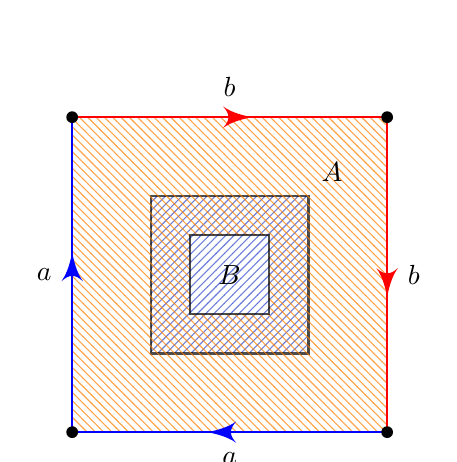
\begin{tikzpicture}
        \draw[pattern=north east lines, opacity=0.7, pattern color=mblue]
          (-1,-1) rectangle (1,1);
        \draw[pattern=north west lines, opacity=0.7, pattern color=orange, even odd rule]
          (-2,-2) rectangle (2,2)        % Outer square
          (-0.5,-0.5) rectangle (0.5,0.5); % Inner square (hole)
        \draw[->-=4/0.8,red] (-2,2) -- (2,2);
        \draw[->-=4/0.8,red] (2,2) -- (2,-2);
        \draw[->-=4/0.8,blue] (2,-2) -- (-2,-2);
        \draw[->-=4/0.8,blue] (-2,-2) -- (-2,2);
        \node[fill, circle, inner sep=1.5pt] (r1) at (-2,-2) {};
        \node[fill, circle, inner sep=1.5pt] (r2) at (2,2) {};
        \node[fill, circle, inner sep=1.5pt] (r3) at (2,-2) {};
        \node[fill, circle, inner sep=1.5pt] (r4) at (-2,2) {};
        \node[label=left:$a$] (a1) at (-2,0) {};
        \node[label=right:$b$] (a2) at (2,0) {};
        \node[label=above:$b$] (b1) at (0,2) {};
        \node[label=below:$a$] (b2) at (0,-2) {};
        \node[label=center:$A$] (A) at (1.3,1.3) {};
        \node[label=center:$B$] (B) at (0,0) {};
      \end{tikzpicture}
      \end{center}
      From the Mayer--Vietoris sequence we get the following
      long exact sequence:
      \[
        \begin{tikzcd}
          \cdots \ar[r] &
          \widetilde H_2(K) \ar[r] & 
          \widetilde H_1(A \cap B) \ar[r] &
          \widetilde H_1(A) \oplus \widetilde H_1(B)
            \ar[out=0, in=180, looseness=2, overlay, lld]\\
          & \widetilde H_1(K) \ar[r]
          & \widetilde H_0(A \cap B) \ar[r]
          & \widetilde H_0(A) \oplus \widetilde H_0(B) \ar [r] & \cdots
        \end{tikzcd}
      \]
      We are already familiar with these groups and can rewrite
      the sequence as:
      \[
        \begin{tikzcd}[ampersand replacement=\&,cramped]
        \widetilde H_2(K) \&
        \Z \& \Z^2 \oplus \set{0} \&
        \widetilde H_1(K) \& 0 \& 0
        \arrow["\delta",from=1-1, to=1-2]
        \arrow["\alpha",from=1-2, to=1-3]
        \arrow["\beta",from=1-3, to=1-4]
        \arrow["\gamma",from=1-4, to=1-5]
        \arrow[from=1-5, to=1-6]
        \end{tikzcd}
      \]
      and by a computation we can see that $\alpha([1]) = ([(2,0)],[0])$.
      From exactness at $\widetilde H_2(K)$ we know that
      $\delta$ is injective, and since $\im \delta = \ker \alpha = 0$,
      we must have $H_2(T^2) = 0$.
      From exactness at $\widetilde H_1(K)$,
      we get that $\widetilde H_1(K) = \im \beta$.
      From the first isomorphism theorem and exactness at $\Z^2$ we get
      \[
        \im \beta \cong
        \frac{\Z^2}{\ker \beta} \cong
        \frac{\Z^2}{\im \alpha} =
        \frac{\Z^2}{2\Z \oplus \set{0}} = \Z/2\Z \oplus \Z,
      \]
      so $\widetilde H_1(K) = \Z/2\Z \oplus \Z$.
      Therefore, by all previous calculations we get:
      \[
        \widetilde H_n(K) =
        \begin{cases}
          0 & n = 0, \\
          \Z/2\Z \oplus \Z & n = 1, \\
          0 &\text{otherwise}.
        \end{cases}
      \]
  \end{enumerate}
\end{solution}

\begin{exercise}
  Let $A \subseteq X$ be topological spaces.
  Prove that the following are equivalent:
  \begin{itemize}
    \item The inclusion $i \colon A \hookrightarrow X$ induces isomorphisms
      $H_n(A) \to H_n(X)$ for all $n$.
    \item The relative groups $H_n(X,A) = 0$ for all $n$.
  \end{itemize}
\end{exercise}
\begin{solution}
  For $(A,X)$ we have the long exact sequence:
  \[\begin{tikzcd}[ampersand replacement=\&,cramped]
    \cdots \& {H_{n+1}(X,A)} \& {H_n(A)} \& {H_n(X)} \& {H_n(X,A)} \& {H_{n-1}(A)} \& \cdots
    \arrow["{q_*}", from=1-1, to=1-2]
    \arrow["\partial", from=1-2, to=1-3]
    \arrow["{i_*}", from=1-3, to=1-4]
    \arrow["{q_*}", from=1-4, to=1-5]
    \arrow["\partial", from=1-5, to=1-6]
    \arrow["{i_*}", from=1-6, to=1-7]
  \end{tikzcd}\]
  If $H_{n+1}(X,A) = H_n(X,A) = 0$,
  then from the exactness of the sequence we get that the map
  $i_* \colon H_n(A) \to H_n(X)$ is an isomorphism.
  On the other hand, if $i_*$ is an isomorphism,
  from the exactness of the sequence
  we get $\im \partial = \ker i_* = \set{0}$, and $\ker \partial = \im q_*$.
  From exactness at $H_n(X)$ we get $\ker q_* = \im i_* = H_n(X)$,
  so $\im q_* = \set{0}$.
  Therefore $\ker \partial = \set{0}$,
  and thus from the first isomorphism theorem
  \[
    \im \partial \cong
    \frac{H_n(X,A)}{\ker \partial} =
    H_n(X,A),
  \]
  so $H_n(X,A) = 0$.
  This holds for arbitrary $n$, so the proof is complete.
\end{solution}

\begin{exercise}
  Prove that $H_n([0,1],A)$ and $\widetilde H_n([0,1]/A)$
  are not isomorphic for the set $A := \set{0} \cup \set{1/n \mid n \in \N}$.
\end{exercise}
\begin{solution}
  First we will compute $H_n([0,1],A)$.
  From the long exact sequence of the pair $([0,1],A)$
  we get the exact sequence:
  \[\begin{tikzcd}[ampersand replacement=\&,cramped]
    0 \& {H_1(X,A)} \& {H_0(A)} \& {H_0(X)} \& {H_0(X,A)} \& 0
    \arrow[from=1-1, to=1-2]
    \arrow[from=1-2, to=1-3]
    \arrow["{i_*}", from=1-3, to=1-4]
    \arrow["{q_*}",from=1-4, to=1-5]
    \arrow[from=1-5, to=1-6]
  \end{tikzcd}\]
  Considering the fact that $X$ is a contractible space,
  and that $A$ is a totally disconnected space with $\N$
  components we can rewrite the sequence as follows:
  \[\begin{tikzcd}[ampersand replacement=\&,cramped]
    0 \& {H_1(X,A)} \& \bigoplus_{m=0}^{\infty} \Z \& \Z \& {H_0(X,A)} \& 0
    \arrow[from=1-1, to=1-2]
    \arrow[from=1-2, to=1-3]
    \arrow["{i_*}", from=1-3, to=1-4]
    \arrow["{q_*}",from=1-4, to=1-5]
    \arrow[from=1-5, to=1-6]
  \end{tikzcd}\]
  Since $i_*$ is induced by the inclusion $A \hookrightarrow X$,
  and by the definition of the spaces,
  we get that $i_*$ is surjective,
  so $q_*$ is the zero map,
  so by exactness at $H_0(X,A)$ we get $H_0(X,A) = \set{0}$.
  From a similar argument in the other direction it's easy to verify
  that $H_1(X,A) = \ker i_* = \bigoplus_{m=1}^{\infty}$.
  Therefore,
  \[
    H_n(X,A) =
    \begin{cases}
      \bigoplus_{m=1}^{\infty} &n = 1, \\
      0 &\text{otherwise}. \\
    \end{cases}
  \]
  Since $X \setminus A$ is the disjoint union of open intervals
  $(\frac{1}{n+1},\frac{1}{n})$, and we collapse $A$ to a point,
  we get that $X/A$ is a space that is homeomorphic to the Hawaiian earring. 
  \begin{figure}[H]
    \centering
    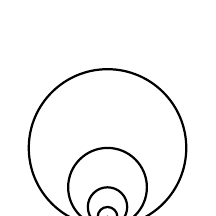
\begin{tikzpicture}[every path/.style={thick}]
      \draw (0,1) circle (1);
      \draw (0,0.5) circle (0.5);
      \draw (0,0.25) circle (0.25);
      \draw (0,0.125) circle (0.125);
      \draw (0,0.125/2) circle (0.125/2);
      \draw (0,0.125/4) circle (0.125/4);
    \end{tikzpicture}
    \caption{The Hawaiian earring.}
  \end{figure}
  However, since for any binary sequence $a_n \in \set{0,1}^{\N}$
  we can create a loop going $a_n$ times around the $n$th circle
  in $X/A$, we get that
  there is a natural surjection from $\pi_1(X/A)$ to $\set{0,1}^{\N}$.
  This implies that $H_1(X/A)$ is uncountable,
  and in particular $H_1(X/A) \neq H_1(X,A)$.
  This completes the proof.
  [A more detailed explanation can be found in Example 1.25 in Hatcher] 
\end{solution}


\section{Simplicial vs Singular homology}

\begin{exercise}
  For a $\Delta$-complex $X$,
  show that the map $\bigsqcup_{\alpha} \sigma_{\alpha} \colon
    \bigsqcup_{\alpha} \Delta^k_{\alpha} \to X^{(k)}$
    (where $\alpha$ runs over the $k$-simplices of $X$)
  induces a homeomorphism $\bigsqcup_{\alpha} \Delta^k_{\alpha} /
  \bigsqcup_{\alpha} \partial \Delta^k_{\alpha} \to X^{(k)} / X^{(k-1)}$.
  Deduce that $X^{(k)} / X^{(k-1)}$ is homeomorphic to a wedge of
  $k$-spheres $\bigvee_{\alpha} S^k$.
\end{exercise}
\begin{solution}

\end{solution}

\begin{exercise}
  Fill in the details  of the proof sketch that simplicial and singular
  homologies are the same.
  Namely, let $X$ be a $\Delta$-complex.
  Prove:
  \begin{enumerate}
    \item[(1)] Every compact set meets the interiors of only finitely many
      simplices in $X$.
    \item[(2)] Prove that the map $H_{n}^{\Delta}(X) \to H_n(X)$
      is an isomorphism (using that $H_{n}^{\Delta}(X^{(k)}) \to H_n(X^{(k)})$)
      is an isomorphism for all $k$).
  \end{enumerate}
\end{exercise}
\begin{solution}

\end{solution}

\begin{exercise}
  Let $X$ be a $\Delta$-complex
  and let $A \subseteq X$ be a subcomplex.
  Prove that $H_{n}^{\Delta}(X,A) \cong H_n(X,A)$.
  [Hint: long exact sequence].
\end{exercise}
\begin{solution}
  We know that the inclusion maps
  $i_X \colon C^{\Delta}_n(X) \to C_n(X)$
  and $i_A \colon C^{\Delta}_n(A) \to C_n(A)$
  induce isomorphisms in their respective homologies.
  From the long exact sequence of pairs we get the following
  diagram:
  \[\begin{tikzcd}[ampersand replacement=\&,cramped]
    \cdots \& {H_n^{\Delta}(A)} \& {H_n^{\Delta}(X)} \& {H_n^{\Delta}(X,A)} \& {H_{n-1}^{\Delta}(A)} \& {H_{n-1}^{\Delta}(X)} \& \cdots \\
    \cdots \& {H_n(A)} \& {H_n(X)} \& {H_n(X,A)} \& {H_{n-1}(A)} \& {H_{n-1}(X)} \& \cdots
    \arrow[from=1-1, to=1-2]
    \arrow[from=1-2, to=1-3]
    \arrow["{{i_A}_*}", from=1-2, to=2-2]
    \arrow[from=1-3, to=1-4]
    \arrow["{{i_X}_*}", from=1-3, to=2-3]
    \arrow[from=1-4, to=1-5]
    \arrow["{{i_{X,A}}_*}", from=1-4, to=2-4]
    \arrow[from=1-5, to=1-6]
    \arrow["{{i_A}_*}", from=1-5, to=2-5]
    \arrow[from=1-6, to=1-7]
    \arrow["{{i_X}_*}", from=1-6, to=2-6]
    \arrow[from=2-1, to=2-2]
    \arrow[from=2-2, to=2-3]
    \arrow[from=2-3, to=2-4]
    \arrow[from=2-4, to=2-5]
    \arrow[from=2-5, to=2-6]
    \arrow[from=2-6, to=2-7]
  \end{tikzcd}\]
  From the five lemma we get that $H_n^{\Delta}(X,A) \cong H_n(X,A)$,
  which completes the proof.
\end{solution}


\section{Degree and cellular homology}

\begin{exercise}
  \label{ex:three-one}
  Given a map $f \colon X \to Y$ we define $S(f)$ to be the map
  $S(X) \to S(Y)$ induced from the map $X \times [-1,1] \to Y \times [-1,1]$
  by $(x,t) \mapsto (f(x),t)$.
  Prove that if $f \colon S^n \to S^n$ has degree $d$,
  then the map $S(f) \colon S(S^n) \to S(S^n)$ has degree $d$.
\end{exercise}
\begin{solution}
  We know that $S(S^n) = S^{n+1}$.
  Denote the two hemispheres of $S(S^n)$ (and some more) by $A$
  and $B$
  Note that $A \cap B$ has a deformation retraction to the equator,
  which is $S^{n}$.
  Since $\mathring A \cup \mathring B = S(S^n)$ we can apply the Mayer--Vietoris
  theorem and get the sequence
  \[\begin{tikzcd}[ampersand replacement=\&,cramped]
    {H_{n+1}(A \cap B)} \& {H_{n+1}(A) \oplus H_{n+1}(B)} \& {H_{n+1}(S^{n+1})} \& {H_{n-1}(A \cap B)} \& 0 \\
    {H_{n+1}(A \cap B)} \& {H_{n+1}(A) \oplus H_{n+1}(B)} \& {H_{n+1}(S^{n+1})} \& {H_{n-1}(A \cap B)} \& 0
    \arrow[from=1-1, to=1-2]
    \arrow["{S(f)_*}", from=1-1, to=2-1]
    \arrow[from=1-2, to=1-3]
    \arrow["{S(f)_*}", from=1-2, to=2-2]
    \arrow["\sim", from=1-3, to=1-4]
    \arrow["{S(f)_*}", from=1-3, to=2-3]
    \arrow[from=1-4, to=1-5]
    \arrow["{S(f)_*}", from=1-4, to=2-4]
    \arrow[from=2-1, to=2-2]
    \arrow[from=2-2, to=2-3]
    \arrow["\sim", from=2-3, to=2-4]
    \arrow[from=2-4, to=2-5]
  \end{tikzcd}\]
  which is equivalent to the sequence
  \[\begin{tikzcd}[ampersand replacement=\&,cramped]
    {H_{n+1}(S^n)} \& {H_{n+1}(A) \oplus H_{n+1}(B)} \& {H_{n+1}(S^{n+1})} \& {H_{n}(S^n)} \& 0 \\
    {H_{n+1}(S^n)} \& {H_{n+1}(A) \oplus H_{n+1}(B)} \& {H_{n+1}(S^{n+1})} \& {H_{n}(S^n)} \& 0
    \arrow[from=1-1, to=1-2]
    \arrow["{S(f)_*}", from=1-1, to=2-1]
    \arrow[from=1-2, to=1-3]
    \arrow["{S(f)_*}", from=1-2, to=2-2]
    \arrow["\sim", from=1-3, to=1-4]
    \arrow["{S(f)_*}", from=1-3, to=2-3]
    \arrow[from=1-4, to=1-5]
    \arrow["{S(f)_*}", from=1-4, to=2-4]
    \arrow[from=2-1, to=2-2]
    \arrow[from=2-2, to=2-3]
    \arrow["\sim", from=2-3, to=2-4]
    \arrow[from=2-4, to=2-5]
  \end{tikzcd}\]
  The diagram commutes by the naturality of the Mayer--Vietoris sequence,
  and therefore,
  $f = r \circ S(f) \circ i$ (where $i$ is the inclusion map
  from $S^n$ to $S(S^n)$ and $r$ is the deformation retract map from
  $S(S^n)$ to the equator $S^n$), and thus $f_* = r_* \circ S(f)_* \circ i_*$,
  where $i_*$ and $r_*$ are isormosphisms.
  Define $1 \in H_n(A \cap B)$ by $i_*(1)$ so
  $r_*(1) = 1$, and thus $S(f)_*(1) = d$,
  so $S(f)$ has degree $d$, which completes the proof.
\end{solution}

\begin{exercise}
  Consider a nonconstant monic polynomial
  $f(z) = z^k + a_{k-1} z^{k-1} + \cdots + a_0$ (where $k > 0$).
  Show that
  \begin{enumerate}
    \item[(1)] $f$ defines a continuous map $f \colon
      S^2 \cong \C \cup \set{\infty} \to \C \cup \set{\infty} \cong S^2$.
    \item[(2)] As such, $f$ is homotopic to the map $f(z) = z^k$.
    \item[(3)] Show that $\deg(f) = k$.
    \item[(4)] Deduce that $f$ is surjective (that's the fundamental theorem
      of algebra!)
  \end{enumerate}
\end{exercise}
\begin{solution} \phantom{}
  \begin{enumerate}
    \item[(1)] Recall that continuity is a local property,
      so $f$ is continuous at $x \in \C$ since its a polynomial,
      and it is continuous at $\infty$ since
      $\lim_{\abs{z} \to \infty} f(z) = \infty$.
    \item[(2)] We can show that $f$ is homotopic to $z \mapsto z^k$
      by defining the following homotopy:
      \[
        H(z,t) := z^k + t(a_{k-1} z^{k-1} + \cdots + a_0).
      \]
      This map is continuous since it's a polynomial in $z$,
      and it clearly a homotopy from $f$ to $z^k$,
      so they have the same degree.
    \item[(3)] Define the map
      \[
        h(z) :=
        \begin{cases}
          \frac{z^k}{\abs{z^k}} &z \neq 0, \\
          0 &z = 0.
        \end{cases}
      \]
      This map is continuous and thus the map
      \[
        H(z,t) = t h(z) + (1 - t) z^k,
      \]
      is a continuous homotopy between $z \mapsto z^k$ and $h$.
      Let $L$ and $U$ be the lower and upper hemispheres of
      $S^2 \cong \C \cup \set{\infty}$ (``and some more'')resepctively,
      and let $r$ be the deformation retraction of $A \cap B$ to $S^1$.
      Then if $i \colon S^1 \hookrightarrow S^2$ is the inclusion map
      of the equator of $S^2$ to $S^2$ we get that
      $r \circ h \circ i \colon S^1 \to S^1$ is simply the map
      $h$ restricted to $S^1$.
      We know that $\deg\del{h\vert_{S^1}} = k$,
      and therefore $r_* \circ h_* \circ i_*$ has degree $k$,
      but by a similar argument to \Cref{ex:three-one},
      since both $i$ and $r$ have degree $1$,
      we must have $\deg(h) = k$.
      Then from part $(2)$ of this exercise $\deg(f) = \deg(h) = k$.
    \item[(4)] If $f$ is not surjective,
      then by properties of the degree $\deg(f) = 0$,
      which is a contradiction so $f$ must be surjective.
  \end{enumerate}
\end{solution}

\begin{exercise}
  Identify $S^3 = \{(x,y) \in \C^2 \mid
    x,y \in \C \stand \norm{x}^2 + \norm{y}^2 = 1\} \subseteq \C^2$.
  For $p,q \in \Z$ let $\alpha \colon S^3 \to S^3$ be the map given by
  $(x,y) \mapsto (e^{2\pi i/p}x, e^{2\pi i p/q}y)$.
  Define $X_{p,q} := S^3/x \sim \alpha(x) \forall x \in S^3$.
  [Hint:
  consider a CW complex structure on $S^3$ whose $1$-skeleton is the circle
  $\set{0} \times S^1 \subseteq S^3$ and whose vertices are
  $(0,e^{2\pi i n/p})$ for $n=1,\dots,p$,
  and is invariant under the action of $\alpha$,
  then compute its quotient.]
\end{exercise}
\begin{solution}

\end{solution}

\begin{exercise}
  Prove that for every map $f \colon S^{2n} \to S^{2n}$ there exists
  $x \in S^{2n}$ such that $f(x) = x$ or $f(x) = -x$.
  Deduce that any map $f \colon \RP^{2n} \to \RP^{2n}$ has a fixed point.
\end{exercise}
\begin{solution}
  Assume without loss of generality that $f(x) \notin \set{x,-x}$
  for all $x \in S^2$.
  This implies that the line connecting $x$ and $f(x)$ is well defined
  and does not intersect with the origin, so the following map is well
  defined:
  \[
    H(x,t) := \frac{(1 - t) f(x) + t x}{\norm{(1 - t) f(x) + t x}}.
  \]
  This map is clearly a homotopy between $f$ and the identity map $\id$.
  This implies that $\deg(f) = 1$.
  However, by properties of degree mappings if $f$ has no fixed points
  then $\deg(f) = (-1)^{2n + 1} = -1$.
  This contradiction completes the proof.

  Next let $f \colon \RP^2 \to \RP^2$ be any map.
  We know that $S^2$ is the universal covering space of $\RP^2$,
  so there exists a unique lift:
  \[\begin{tikzcd}[ampersand replacement=\&,cramped]
    {S^{2n}} \& {S^{2n}} \\
    {\RP^{2n}} \& {\RP^{2n}}
    \arrow["{\tilde f \circ q}", from=1-1, to=1-2]
    \arrow["q", from=1-1, to=2-1]
    \arrow["q", from=1-2, to=2-2]
    \arrow["{\tilde f}", from=2-1, to=1-2]
    \arrow["f", from=2-1, to=2-2]
  \end{tikzcd}\]
  The map $\tilde f \circ q$ satisfies the conditions of the exercise,
  so there must exist $x \in S^{2n}$ so that $\tilde f \circ q(x) = x$,
  or $\tilde f \circ q(x) = -x$.
  Without loss of generality assume that $\tilde f \circ q(x) = x$.
  Then by the commutativity of the diagram
  we get
  \[
    f(x) =
    f([\pm x]) =
    q \circ \tilde f \circ q(x) =
    q(x) =
    [\pm x],
  \]
  so $f$ has a fixed point, which completes the proof.
\end{solution}

\begin{exercise}
  Prove Brouwer's fixed point theorem for a function $f \colon \D^n \to \D^n$,
  by using a degree map $\tilde f \colon S^n \to S^n$ that sends both
  the northern and southern hemispheres to the northern hemisphere via $f$.
\end{exercise}
\begin{solution}
  Define $\phi \colon S^n \to \D^n$ by
  $\phi(x_0,\dots,x_n) = (x_0,\dots,x_{n-1})$,
  and $\psi \D^n \to (S^n)^+$ by
  $\psi(\vec y) = \psi(y_1,\dots,y_n) =
  (y_1,\dots,y_n,(1-\norm{\vec y}^2)^{1/2})$,
  where $(S^n)^+$ denotes the northern hemisphere with boundary.
  Next consider the map $\tilde f = \psi \circ f \circ \phi \colon S^n \to S^n$.
  This map is certainly not onto since the southern pole in $S^n$
  has no preimage. Therefore $\deg(\tilde f) = 0$.
  A degree map with no fixed point has degree $(-1)^{n+1}$,
  and therefore $\tilde f$ must have a fixed point.
  Since $\tilde f$'s image is in $(S^n)^+$, the fixed point must be a point
  $p \in (S^n)^+$ and we can write $\psi \circ f \circ \phi(p) = p$.
  The map $\psi$ is a bijection,
  so we can write $f \circ \phi(p) = \psi^{-1}(p)$.
  We can also notice that $q := \psi^{-1}(p) = \phi(p)$,
  and now we get $f(q) = q$,
  so $f$ has a fixed point, which completes the proof.
\end{solution}

\begin{exercise}
  \label{ex:snf-homologies}
  compute the homologies of the space $x := [0,1]^{3} / \sim$
  where $\sim$ is the equivalence relation identifying each face of the cube
  with its opposite face by a $\pi/2$-clockwise-rotation.
\end{exercise}
\begin{solution}
  The space $X$ we are working with looks something like this:
  \begin{center}
  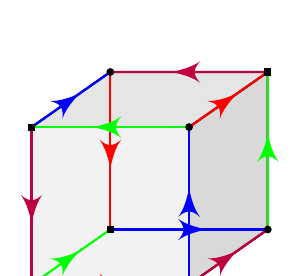
\begin{tikzpicture}[scale=2, line cap=round, line join=round]
  % front square
  \coordinate (A) at (0,0);
  \coordinate (B) at (1,0);
  \coordinate (C) at (1,1);
  \coordinate (D) at (0,1);
  % back square (shifted)
  \coordinate (shift) at (0.5,0.35);
  \coordinate (E) at ($(A)+(shift)$);
  \coordinate (F) at ($(B)+(shift)$);
  \coordinate (G) at ($(C)+(shift)$);
  \coordinate (H) at ($(D)+(shift)$);

  % faces (optional shading)
  \fill[gray!10] (A)--(B)--(C)--(D)--cycle;         % front
  \fill[gray!20] (D)--(C)--(G)--(H)--cycle;         % top
  \fill[gray!30] (B)--(C)--(G)--(F)--cycle;         % right

  % visible edges
  \draw (A)--(B)--(C)--(D)--cycle;
  \draw (B)--(F)--(G)--(C);
  \draw (D)--(H)--(G);

  \draw[->-=2,red] (H) -- (E);
  \draw[->-=2,blue] (E) -- (F);
  \draw[->-=2,green] (F) -- (G);
  \draw[->-=2,purple] (G) -- (H);

  \draw[->-=2,purple] (B) -- (F);
  \draw[->-=2,green] (A) -- (E);
  \draw[->-=2,blue] (D) -- (H);
  \draw[->-=2,red] (C) -- (G);

  \draw[->-=2,red] (A) -- (B);
  \draw[->-=2,blue] (B) -- (C);
  \draw[->-=2,green] (C) -- (D);
  \draw[->-=2,purple] (D) -- (A);
  \node[fill, circle, inner sep=1.0pt] (v) at (A) {};
  \node[fill, rectangle, inner sep=1.3pt] (v) at (B) {};
  \node[fill, circle, inner sep=1.0pt] (v) at (C) {};
  \node[fill, rectangle, inner sep=1.3pt] (v) at (D) {};
  \node[fill, rectangle, inner sep=1.3pt] (v) at (E) {};
  \node[fill, circle, inner sep=1.0pt] (v) at (F) {};
  \node[fill, rectangle, inner sep=1.3pt] (v) at (G) {};
  \node[fill, circle, inner sep=1.0pt] (v) at (H) {};
\end{tikzpicture}
  \end{center}
  This is a CW-complex with two $0$-cells
  (let the circle vertices form the equivalence class $p$
  and the rest can form the equivalence class $q$), four $1$-cells
  (denote the red edge by $a$, the blue by $b$, the green by $c$,
  and the purple by $d$),
  three $2$-cells (denote the front/back faces by $f$,
  the left/right faces by $g$, and the bottom/top faces by $h$),
  and one $3$-cell (which represents the interior of the cube.
  We denote it by $T$).
  The cellular chain complex is:
  \[\begin{tikzcd}[ampersand replacement=\&,cramped]
    0 \& {\langle T \rangle} \& {\langle f,g,h \rangle} \& {\langle a,b,c,d \rangle} \& {\langle p,q \rangle} \& 0
    \arrow[from=1-1, to=1-2]
    \arrow["{d_3}", from=1-2, to=1-3]
    \arrow["{d_2}", from=1-3, to=1-4]
    \arrow["{d_1}", from=1-4, to=1-5]
    \arrow[from=1-5, to=1-6]
  \end{tikzcd}\]
  We can easily compute the boundary maps $d_1$ and $d_2$
  by using local degree,
  and efficiently write their values in the tables below:
  \[
    d_1 = \left[ \begin{array}{c|cccc}
    & a & b & c & d \\ \hline
    p & -1 & 1  & -1 & 1 \\
    q & 1  & -1 & 1  & -1
    \end{array} \right]
    \tand
    d_2 = \left[ \begin{array}{c|ccc}
    & f & g & h \\ \hline
    a & 1 & 1  & 1 \\
    b & 1 & 1  & -1 \\
    c & 1 & -1 & -1 \\
    d & 1 & -1 & 1
    \end{array} \right]
  \]
  By using the cellular boundary formula we get that
  \[
    d_3(T) = \sum_{\alpha = f}^{h} \deg(\varphi_{T \alpha}) \alpha. 
  \]
  We are going to compute $\deg(\varphi_{T \alpha})$ using local degrees.
  We know that the preimage of any point in $\alpha$ (some face of $X$)
  has two preimages in $T$.
  For example the center point of $f$ has the center points of the
  front and back faces of $T$.
  Neighbourhoods of these points are mapped homeomorphically onto a
  neighbourhood of the image, so the local degree at each point is $\pm 1$.
  Since each neighbourhood differs by a rotation and reflection from the
  other, their degrees differ by a sign (rotation doesn't change the
  degree and reflection is multiplication by $-1$),
  so we can conclude that $\deg(\varphi_{T \alpha}) = 1 - 1 = 0$.
  Since this is true for all $\alpha$, we get
  \[
    d_3(T) = \sum_{\alpha = f}^{h} \deg(\varphi_{T \alpha}) \alpha = 0. 
  \]
  We can now compute the homologies directly,
  but I prefer to introduce a different approach to computing the homologies
  of the space, which is way more efficient.
  The way is introduced in \Cref{sec:computing-homology},
  so read that before continuing.

  It is very easy to
  find the smith normal forms of the linear maps
  $d_1$ and $d_2$ (you can even do this in your head, and if you can't
  make sure you know how to find the SNF again),
  they are:
  \[
    d_1 \taking{\text{SNF}}
    \begin{pmatrix}
      1 & 0 & 0 & 0 \\
      0 & 0 & 0 & 0
    \end{pmatrix}
    \tand
    d_2 \taking{\text{SNF}}
    \begin{pmatrix}
      1 & 0 & 0 \\
      0 & 2 & 0 \\
      0 & 0 & 2 \\
      0 & 0 & 0
    \end{pmatrix}.
  \]
  By the formula from \Cref{prop:fast-homology} we get:
  \begin{align*}
    &H_0(X) \cong \Z \\
    &H_1(X) \cong \Z/2\Z \oplus \Z/2\Z \\
    &H_2(X) \cong 0 \\
    &H_3(X) \cong \Z
  \end{align*}
\end{solution}

\begin{exercise}
  \label{ex:three-nineteen}
  Let $q \colon S^n \to \RP^{n} = S^n/x \sim -x, \forall x \in S^n$
  be the quotient map.
  Compute $q_* \colon H_n(S^n) \to H_n(\RP^n)$.
\end{exercise}
\begin{solution}
  We know that when $n$ is even, that $H_n(\RP^n) = 0$,
  so $q_*$ must be the zero map.

  Let $n$ be an odd natural number, so that $n = 2k + 1$
  for some $k \in \N$.
  We know that in this case $H_n(\RP^{2k + 1}) = \Z$,
  and we also have the following chain complex
  for $\RP^{2k + 2}$:
  \[\begin{tikzcd}[ampersand replacement=\&,cramped]
    \cdots \& \Z \& \Z \& \cdots \& \Z \& \Z \& 0
    \arrow["d_{2k+2}", from=1-1, to=1-2]
    \arrow["0", from=1-2, to=1-3]
    \arrow["2", from=1-3, to=1-4]
    \arrow["2", from=1-4, to=1-5]
    \arrow["0", from=1-5, to=1-6]
    \arrow["0", from=1-6, to=1-7]
  \end{tikzcd}\]
  where $d_{2k+2}$ is also the map $d_{2k+2} = 2$.
  Note that $d_{2k+2} = (p \circ q)_*$
  for the map $p \colon \RP^{2k+1} \to \RP^{2k+1}/\RP^{2k} \cong S^n$,
  and thus $\deg(p \circ q) = 2$.
  Since the pair $(\RP^{2k+1},\RP^{2k})$ is a good pair we get the exact
  sequence:
  \[\begin{tikzcd}[ampersand replacement=\&,cramped]
    {H_{2k+1}(\RP^{2k})} \& {H_{2k+1}(\RP^{2k+1})} \& {H_{2k+1}(S^{2k+1})} \& {H_{2k}(\RP^{2k})}
    \arrow[from=1-1, to=1-2]
    \arrow[from=1-2, to=1-3]
    \arrow[from=1-3, to=1-4]
  \end{tikzcd}\]
  where both ends are trivial so we have the isomorphism
  $H_{2k+1}(\RP^{2k+1}) \cong H_{2k+1}(S^{2k+1})$.
  Since both groups are $\Z$, we must have $p_*(1) = \pm 1$
  depending on the choice of generator of $\RP^{2k+1}$.
  Choose generator so that $p_*(1) = 1$,
  and then from multiplicity of the degree we get $\deg(q) = 2$
  (in other words $q_*(1) = 2$).
  This completes the proof.
\end{solution}

\begin{exercise}
  Prove that if $f \colon S^n \to S^n$ is even ($f(x) = f(-x)$),
  then $\deg(f)$ is even.
  [Hint: use \Cref{ex:three-nineteen}]
\end{exercise}.
\begin{solution}
  If $f$ is even then $f$ is constant on the equivalence classes
  of $\RP^2$ and thus we have the following commutative diagram:
  \[\begin{tikzcd}[ampersand replacement=\&,cramped]
    {\RP^2} \\
    {S^n} \& {S^n}
    \arrow["{\tilde f}", from=1-1, to=2-2]
    \arrow["q", from=2-1, to=1-1]
    \arrow["f"', from=2-1, to=2-2]
  \end{tikzcd}\]
  so $(\tilde f \circ q)_* = f_*$,
  and from functoriality of the induced map we get that
  $f_* = \tilde f_* \circ q_*$.
  We therefore have that $\deg(f) = \deg(\tilde f) \deg(q)$,
  but by \Cref{ex:three-nineteen} we know that $\deg(q)$
  is either $0$ or $2$ so $\deg(f)$ must be even,
  which completes the proof.
\end{solution}


\section{Splitting lemma and dual groups}
\begin{exercise}
  Prove the splitting lemma:
  Let
  \[\begin{tikzcd}[ampersand replacement=\&,cramped]
    0 \& A \& B \& C \& 0
    \arrow[from=1-1, to=1-2]
    \arrow["\alpha", from=1-2, to=1-3]
    \arrow["\beta", from=1-3, to=1-4]
    \arrow[from=1-4, to=1-5]
  \end{tikzcd}\]
  be a short exact sequence of abelian groups.
  Then the following are equivalent:
  \begin{enumerate}
    \item[(1)] There exists $s \colon C \to B$ such that $\beta s = \id_C$.
    \item[(2)] There exists $r \colon B \to A$ such that $r \alpha = \id_A$.
    \item[(3)] We have $B \cong A \oplus C$, and the maps $\alpha$, $\beta$
      are the natural inclusion and projection maps.
  \end{enumerate}
\end{exercise}
\begin{solution}
  The directions $(3 \to 1)$ and $(3 \to 2)$ are obvious,
  so we will only show directions $(1 \to 2)$ and $(2 \to 3)$.
  \begin{enumerate}
    \item[$(1 \to 2)$] Let $b \in B$, then $\beta(s\beta b - b) = 0$,
      so by exactness $(s\beta b - b) \in \ker(\beta) = \im(\alpha)$.
      Since $\alpha$ is injective there exists a unique $a \in A$
      such that $\alpha(a) = s\beta b - b$.
      We define $r \colon B \to A$ by $r(b) := a$.
      In this way we have $r\alpha(a) = a$ so $r\alpha = \id_A$
      and it is left to show that $r$ is a homomorphism.
      Denote $r(b_1 + b_2) = a$, $r(b_1) = a_1$ and $r(b_2) = a_2$.
      We now have from previous definitions that
      \[
        \alpha(a - (a_1 + a_2)) =
        s\beta (b_1 + b_2) - (b_1 + b_2) -
        (s\beta (b_1 + b_2) - (b_1 + b_2)) = 0,
      \]
      but $\alpha$ is injective so $a - (a_1 + a_2) = 0$,
      which means that $a = a_1 + a_2$, which completes this part of the proof.
    \item[$(2 \to 3)$] Define $\varphi \colon B \to C \oplus A$ by
      $\varphi(b) = (\beta(b),r(b))$.
      The map $\varphi$ is a homomorphism, and we will show that it is
      an isomorphism directly.
      If $b \in \ker(\varphi)$ then $\beta(b) = r(b) = 0$,
      but since $b \in \ker(\beta) = \im(\alpha)$,
      there exists $a$ so that $\alpha a = b$,
      so $r(\alpha a) = r(b) = 0$,
      but also by the assumption $r(\alpha a) = \id_A(a) = a$.
      This implies that $a = 0$, and thus $b = 0$,
      so $\ker(\varphi) = 0$, and $\varphi$ is an injection.
      We will now show surjectivity.
      Let $(c,a) \in C \oplus A$.
      Since $\beta$ is surjective, there exists $b \in B$ so that
      $\beta(b) = c$.
      Since $\im \alpha = \ker \beta$
      and $\alpha(a - r(b)) \in \im(\alpha)$
      we get $\beta(b + \alpha(a - r(b))) = \beta(b) = c$,
      and we also have
      $r(b + \alpha(a - r(b))) = r(b) + (a - r(b)) = a$,
      so $\varphi(b + \alpha(a - r(b))) = (c,a)$,
      which means it is a surjection.
      We have shown that $\varphi$ satisfies all properties of an isomorphism,
      therefore it is an isomorphism.
      \[\begin{tikzcd}[ampersand replacement=\&,cramped]
      \&\& B \\
      0 \& A \&\& C \& 0 \\
      \&\& {A \oplus C}
      \arrow["\beta", from=1-3, to=2-4]
      \arrow["\varphi", from=1-3, to=3-3]
      \arrow["0", from=2-1, to=2-2]
      \arrow["\alpha", from=2-2, to=1-3]
      \arrow["i", from=2-2, to=3-3]
      \arrow["0", from=2-4, to=2-5]
      \arrow["\pi", from=3-3, to=2-4]
    \end{tikzcd}\]
    We have shown that $\varphi$ is an isomorphism.
    Since $\varphi \alpha(a) = r \alpha a = i_A(a)$ for all $a$,
    we get that $\alpha$ is the inclusion map.
    Since $\pi \varphi(b) = \beta(b)$, it is clear that the projection $\pi$
    is $\beta$ (equivalently $\beta$ is the projection),
    which completes the proof.
  \end{enumerate}
\end{solution}

\begin{remark}
  In the following exercises, we fix some $G$ and denote $A^* = \Hom(A,G)$.
\end{remark}

\begin{exercise}
  \label{ex:exact-sequences}
  Prove that if $A \taking{\quad} B \taking{\quad} C \taking{\quad} 0$
  is exact then $0 \taking{\quad} C^* \taking{\quad} B^* \taking{\quad} A^*$
  is exact.
\end{exercise}
\begin{solution}
  First we denote
  \[\begin{tikzcd}[ampersand replacement=\&,cramped]
    A \& B \& C \& 0
    \arrow["\alpha", from=1-1, to=1-2]
    \arrow["\beta", from=1-2, to=1-3]
    \arrow[from=1-3, to=1-4]
  \end{tikzcd}\]
  and
  \[\begin{tikzcd}[ampersand replacement=\&,cramped]
    {A^*} \& {B^*} \& {C^*} \& 0
    \arrow["{\alpha^*}"', from=1-2, to=1-1]
    \arrow["{\beta^*}"', from=1-3, to=1-2]
    \arrow[from=1-4, to=1-3]
  \end{tikzcd}\]
  We are now going to prove exactness at every element of
  the sequence seperately.
  \begin{description}
    \item[$(\ker \beta^* = 0)$]
      Let $\varphi \in \ker \beta^*$.
      This implies that $\beta^*(\varphi(b)) = 0$,
      so by definition of the dual map
      $\beta^* \varphi(b) := \varphi(\beta (b)) = 0$.
      This holds for all $b$, and by assumption $\beta$ is surjective,
      so necessarily $\varphi \equiv 0$.
      This implies that $\ker \beta^* = 0$ and concludes the first part
      of the proof.
    \item[$(\ker \alpha^* = \im \beta^*)$]
      First let $\varphi \in \im \beta^*$,
      then by definition of the dual maps
      we get $\alpha^* \varphi = \alpha^* \beta^* \psi = \psi \beta \alpha$,
      and from exactness $\beta \alpha = 0$
      so all of this just gives $\alpha^* \varphi \equiv 0$
      or $\varphi \in \ker \alpha^*$.
      On the other hand if $\varphi \in \ker \alpha^*$
      define $\psi \colon C \to G$ by $\psi(c) = \varphi(\beta^{-1}(c))$.
      In this way, $\beta^* \psi = \psi \circ \beta = \varphi$,
      so $\varphi \in \im \beta^*$.
      However, we still need to show that $\psi$ is a well defined
      homomorphism.
      Suppose that $b_1,b_2 \in q^{-1}(c)$,
      then $b_1 - b_2 \in \ker \beta = \im \alpha$,
      so there exists $a$ such that $\alpha(a) = b_1 - b_2$.
      Since $\varphi \in \ker \alpha^*$ it is constantly zero on $\ker \beta$,
      so we get
      \[
        0 =
        \varphi(\alpha(a)) =
        \varphi(b_1 - b_2) =
        \varphi(b_1) - \varphi(b_2).
      \]
      This implies that $\varphi(b_1) = \varphi(b_2)$,
      and so $\psi$ is well defined.
      We also need to show that $\psi \in C^*$,
      which means that we need to show it is a homomorphism.
      Indeed
      \[
        \psi(c_1 + c_2) =
        \varphi(q^{-1}(c_1 + c_2)) =
        \varphi(b_1 + b_2) =
        \psi(c_1) + \psi(c_2),
      \]
      where $b_1 \in q^{-1}(c_1)$ and $b_2 \in q^{-1}(c_2)$
      respectively, which completes the proof.
  \end{description}
\end{solution}

\begin{exercise}
  Prove that if
  $0 \taking{\quad} A \taking{\quad} B \taking{\quad} C \taking{\quad} 0$
  splits then
  $0 \taking{\quad} C^* \taking{\quad} B^* \taking{\quad} A^* \taking{\quad} 0$
  splits.
\end{exercise}
\begin{solution}
  By \Cref{ex:exact-sequences} we know that
  $0 \taking{\quad} C^* \taking{\quad} B^* \taking{\quad} A^*$ is exact,
  and therefore we just need to show that $\alpha^*$ is onto.
  Since $B = A \oplus C$, we have $B^* = A^* \oplus C^*$,
  so $\alpha^*$ is the restriction map
  (it takes a map in $(A \oplus C)^*$ and maps it to its restriction
  to $A$, so it is in $A^*$), and clearly the restriction is surjective,
  which completes the proof.
\end{solution}


\section{Cohomology}
\begin{exercise}
 Compute directly (using cellular cohomology) the cohomologies of $\RP^n$
 with coefficient groups $G = \Z/2\Z$ and $G = \Z$.
\end{exercise}
\begin{solution}
  We can consider the standard CW-complex for $\RP^n$ which consists
  of exactly one cell in every dimension.
  We then get that the cellular chain complex is:
  \[\begin{tikzcd}[ampersand replacement=\&,cramped]
    \cdots \& 0 \& \Z \& \cdots \& \Z \& \Z \& \Z \& 0
    \arrow[from=1-1, to=1-2]
    \arrow[from=1-2, to=1-3]
    \arrow["{\partial_n}", from=1-3, to=1-4]
    \arrow["0", from=1-4, to=1-5]
    \arrow["2", from=1-5, to=1-6]
    \arrow["0", from=1-6, to=1-7]
    \arrow["0", from=1-7, to=1-8]
  \end{tikzcd}\]
  where $\partial_n$ multiplies by $2$ if $n$ is even,
  and is the zero map otherwise.
  When $G = \Z/2\Z$ we get by definition
  that $C^n(\RP^n;G) = \Hom(\Z,\Z/2\Z) \cong \Z/2\Z$,
  and that $\delta_k h(x) = h\del{\partial_k(x)} = 0 \cdot h(1) = 0$,
  since $\partial_k(x) \in 2\N$ and thus is equivalent to $0$ in $G$.
  Therefore the dual chain complex is:
  \[\begin{tikzcd}[ampersand replacement=\&,cramped]
    \cdots \& 0 \& {\Z/2\Z} \& {\Z/2\Z} \& \cdots \& {\Z/2\Z} \& 0
    \arrow[from=1-2, to=1-1]
    \arrow["0"', from=1-3, to=1-2]
    \arrow["0"', from=1-4, to=1-3]
    \arrow["0"', from=1-5, to=1-4]
    \arrow["0"', from=1-6, to=1-5]
    \arrow["0"', from=1-7, to=1-6]
  \end{tikzcd}\]
  so the cohomology is simply:
  \[
    H^k(X) =
    \begin{cases}
      \Z/2\Z &0 \le k \le n, \\
      \set{0} &\text{otherwise}.
    \end{cases}
  \]
  When $G = \Z$, we get that $C^n(\RP^n;G) = \Hom(\Z,\Z) \cong \Z$,
  and
  \[
    \delta_k h(x) = h\del{\partial_k(x)} =
    \begin{cases}
      2 h(x) & 1 \le k \le n \stand k \text{ even}, \\
      0 &\text{otherwise}.
    \end{cases}
  \]
  Therefore the dual chain complex is: 
  \[\begin{tikzcd}[ampersand replacement=\&,cramped]
    \cdots \& 0 \& \Z \& \Z \& \cdots \& \Z \& \Z \& 0
    \arrow[from=1-2, to=1-1]
    \arrow["0"', from=1-3, to=1-2]
    \arrow["{\delta_n}"', from=1-4, to=1-3]
    \arrow["2"', from=1-5, to=1-4]
    \arrow["2"', from=1-6, to=1-5]
    \arrow["0"', from=1-7, to=1-6]
    \arrow["0"', from=1-8, to=1-7]
  \end{tikzcd}\]
  Therefore for even $n$ we get
  \[
    H^k(\RP^n) =
    \begin{cases}
      0 &k < n \stand k\text{ odd} \stor k > n, \\
      \Z/2\Z &1 \le k \le n \stand k\text{ even}, \\
      \Z &k = 0.
    \end{cases}
  \]
  And for odd $n$ we get
  \[
    H^k(\RP^n) =
    \begin{cases}
      0 &k < n \stand k\text{ odd} \stor k > n, \\
      \Z/2\Z &1 \le k < n \stand k\text{ even}, \\
      \Z &k = 0 \stor k = n.
    \end{cases}
  \]
\end{solution}

\begin{exercise}
  Repeat the previous exercise using the universal coefficient theorem.
\end{exercise}
\begin{solution}
  When $G = \Z$,
  by a corollary of the universal coefficient theorem we know that:
  \[
    H^k(\RP^n;\Z) \cong
    \text{torsion of } H_{k-1}(\RP^n) \oplus
    \text{free part of } H_{k}(\RP^n).
  \]
  Recall that when $n$ is odd
  \[
    H_k(\RP^n) =
    \begin{cases}
      \Z, &k = 0 \stor k = n, \\
      \Z/2\Z, &0 < k < n \stand \text{$k$ is odd}, \\
      \set{0}, &\text{otherwise}.
    \end{cases}
  \]
  and when $n$ is even
  \[
    H_k(\RP^n) =
    \begin{cases}
      \Z, &k = 0, \\
      \Z/2\Z, &0 < k < n \stand \text{$k$ is odd}, \\
      \set{0}, &\text{otherwise}.
    \end{cases}
  \]
  Therefore, by a matter of simple calculation, when $n$ is odd:
  \[
    H^k(\RP^n;\Z) =
    \begin{cases}
      \Z &k = 0 \stor k = n, \\
      \Z/2\Z &0 < k < n \stand k\text{ even}, \\
      \set{0} &\text{otherwise}.
    \end{cases}
  \]
  and when $n$ is even:
  \[
    H^k(\RP^n;\Z) =
    \begin{cases}
      \Z &k = 0, \\
      \Z/2\Z &0 < k \le n \stand k\text{ even}, \\
      \set{0} &\text{otherwise}.
    \end{cases}
  \]
  and when $G = \Z/2\Z$, we have that $G$ is in particular
  a field, and thus we can use the following fact from the lectures:
  \[
    H^k(\RP^n;\Z/2\Z) =
    \Hom_{\Z/2\Z}(H_k(\RP^n ; \Z/2\Z), \Z/2\Z).
  \]
  Recall that we saw in class that for any $n$, we have that
  \[
    H_k(\RP^n ; \Z/2\Z) =
    \begin{cases}
      \Z/2\Z &0 \le k \le n, \\
      \set{0} &k > n.
    \end{cases}
  \]
  We therefore have for any $n$ and $0 \le k \le n$ that
  \[
    H^k(\RP^n;\Z/2\Z) =
    \Hom_{\Z/2\Z}(\Z/2\Z, \Z/2\Z) = \Z/2\Z.
  \]
  This concludes this exercise since all the other cohomologies are trivial:
  \[
    H^k(\RP^n;\Z/2\Z) =
    \begin{cases}
      \Z/2\Z &0 \le k \le n, \\
      \set{0} &k > n.
    \end{cases}
  \]
\end{solution}


\section{Extra: Computing homology groups efficiently}
\label{sec:computing-homology}
The propositions in this subsection are definitely not mine,
and are were taken from the site of Omar Antol\'in Camarena
(I slightly modified them), for the purpose of showing an extremely
easy way to compute homology groups, which I'm not sure why but we weren't
taught them at class.
However, we were taught about the Smith normal form in the first problem
set, and it is necessary to be familiar with it before continuing to read
the rest of this subsection.

\begin{proposition}
  \label{prop:snf-homology-lemma}
  Let the nonzero elementary divisors of an $m \times n$ integer
  matrix $A$ be denoted by $a_1,a_2,\dots,a_r$
  (so that $r$ is the rank of $A$).
  Then $\coker(A) :=
  \Z^m/\im(A) \cong \bigoplus_{i=1}^{r} \Z/a_i\Z \oplus \Z^{m-r}$.
\end{proposition}
\begin{proof}
  Let $A = UDV$ be the Smith normal form of $A$.
  Then $\coker(A) \cong \coker(D)$
  via the map $x + \im(A) \mapsto U^{-1} x + \im(D)$.
  It is clear that $\coker(D) =
  \Z^m/\im(D) \cong \bigoplus_{i=1}^{r} \Z/a_i\Z \oplus \Z^{m-r}$,
  which completes the proof.
\end{proof}

\begin{proposition}
  \label{prop:fast-homology}
  Given a complex $\Z^n \taking{A} \Z^m \taking{B} \Z^k$ so that $BA = 0$
  (which is exactly the condition $\partial^2 = 0$ we always have),
  the homology at the middle term is given by
  $\ker(B)/\im(A) \cong \bigoplus_{i=1}^{r} \Z/a_i\Z \oplus \Z^{m - r - s}$
  where $r = \rank(A)$, $s = \rank(B)$ and $a_1,\dots,a_r$ are the nonzero
  elementary divisors of $A$.
\end{proposition}
\begin{proof}
  Since $B$ is zero on $\im(A)$, it can be well defined as a map
  $\overline B \colon \Z^m / \im(A) \to \Z^k$.
  We can notice that
  under this notation $\ker(B)/\im(A) \cong \ker(\overline B)$.

  By \Cref{prop:snf-homology-lemma},
  we have $\Z^m/\im(A) \cong \bigoplus_{i=1}^{r} \Z/a_i\Z \oplus \Z^{m-r}$.
  Since the target of $\overline B$ ($\Z^k$) is free,
  all torsion elements in its domain must be sent to zero,
  and are thus in $\ker(\overline B)$, so we see that
  \[
    \ker(\overline B) =
    \bigoplus_{i=1}^{r} \Z/a_i\Z \oplus \ker(\overline B\vert_{\Z^{m-r}}).
  \]
  Since any subgroup of a free abelian group is free,
  the kernel of the restriction of $\overline B$ to the free part
  $\ker(\overline B\vert_{\Z^{m-r}}) \leqslant \Z^{m-r}$ is free,
  and its rank is $m - r - s$, because $s$ is the rank of
  $\im(B) = \im(\overline B) = \im(B\vert_{\Z^{m-r}})$.
  Thus it is $\Z^{m - r - s}$, so
  \[
    \ker(\overline B) =
    \bigoplus_{i=1}^{r} \Z/a_i\Z \oplus \Z^{m - r - s},
  \]
  which completes the proof.
\end{proof}

An example of using this method in can be found in \Cref{ex:snf-homologies}.




\end{document}
